\documentclass[
  ngerman,
  paper=a4,
  10pt,
  headings=small,
  DIV=15,
]{scrartcl}

% use utf-8 encoding.
\usepackage[utf8]{inputenc}

% setup main font.
\usepackage{fontspec}
\setsansfont{Helvetica Neue}[
  BoldFont = {Helvetica Neue Bold},
]
\renewcommand{\familydefault}{\sfdefault}
\usepackage{microtype}

% space to leave in between answers.
\renewcommand{\arraystretch}{1.2}

% question environment (uses a table).
\newenvironment{question}[2]{
  \noindent
  \setcounter{answer}{1}
  \begin{tabular}{@{}cp{6.5cm}@{}}
  \textbf{#1} & \textbf{#2}\\
  \ifcsname #1\endcsname
    Hi & oops\\
  \fi
}{
  \end{tabular}
  \bigskip
}

\newcounter{answer}
\newcommand{\answer}[1]{
  \textbf{\Alph{answer}}
  \stepcounter{answer}
  & #1\\}
  
\usepackage{tikz}
\usetikzlibrary{circuits.ee.IEC}
\usetikzlibrary{positioning}
\newcommand{\graphic}[1]{&#1\\}
\tikzset{
  every circuit symbol/.style={draw,very thick},
  every circuit wire/.style={draw,very thick},
  every circuit/.style={draw,very thick,huge circuit symbols}}


% quotes setup
\usepackage{babel}
\usepackage{csquotes}
\MakeOuterQuote{"}

\title{Prüfungsfragen im Prüfungsteil "Technische Kenntnisse" bei Prüfungen zum Erwerb von Amateurfunkzeugnissen der Klasse E}
\date{September 2006}

\begin{document}
  % title page
  \maketitle
    
  % first page
  \newpage
  \vspace*{\fill}
  \noindent
  Dieser Fragen- und Antwortenkatalog basiert auf §~4 Abs.~1 Amateurfunkgesetz (AFuG) in Verbindung mit §~4 der durch Artikel~1 Ziffer~2 der Ersten Verordnung zur Änderung der Amateurfunkverordnung vom 25.~August 2006 (BGBl.~I~S.~2070) geänderten Verordnung zum Gesetz über den Amateurfunk (AFuV) vom 15. Februar 2005 (BGBl.~I~S.~242) in der Form, wie sie am 1.~Februar 2007 in Kraft tritt. Aus dem Katalog ersichtliche Einzelheiten werden erst ab dem 1.~Februar 2007 bei Amateurfunkprüfungen umgesetzt bzw. angewendet. Dazu erfolgt vor dem 1.~Februar 2007 eine entsprechende Veröffentlichung im Amtsblatt der Bundesnetzagentur.

\bigskip\noindent
Dieser Fragen- und Antwortenkatalog unterliegt den Bestimmungen des §~5 des Urheberrechtsgesetzes (UrhG).
Er kann jederzeit erweitert und aktualisiert werden. Neuauflagen werden im Amtsblatt der Bundesnetzagentur bekannt gegeben.
  \newpage
  \tableofcontents
  \twocolumn
  
  \section{Allgemeine mathematische Grundkenntnisse und Größen}

\subsection{Allgemeine mathematische Grundkenntnisse}

\begin{question}{TA101}{0,042 A entspricht}
\answer{42⋅10-3 A.}
\answer{42⋅103 A.}
\answer{42⋅10-2 A.}
\answer{42⋅10-1 A.}
\end{question}

\begin{question}{TA102}{0,00042 A entspricht}
\answer{420.10-6 A.}
\answer{420.106 A.}
\answer{420.10-5 A.}
\answer{42.10-6 A.}
\end{question}

\begin{question}{TA103}{100 mW entspricht}
\answer{10-1 W.}
\answer{0,001 W.}
\answer{0,01 W.}
\answer{10-2 W.}
\end{question}

\begin{question}{TA104}{4 200 000 Hz entspricht}
\answer{4,2⋅106 Hz.}
\answer{4,2⋅105 Hz.}
\answer{42⋅106 Hz.}
\answer{42⋅10-5 Hz.}
\end{question}

\subsection{Größen und Einheiten}

\begin{question}{TA201}{Welche Einheit wird für die elektrische Spannung verwendet?}
\answer{Volt (V)}
\answer{Ampere (A)}
\answer{Ohm (Ω)}
\answer{Amperestunden (Ah)}
\end{question}

\begin{question}{TA202}{Welche Einheit wird für die elektrische Ladung verwendet?}
\answer{Amperesekunde (As)}
\answer{Kilowatt (kW)}
\answer{Joule (J)}
\answer{Ampere (A)}
\end{question}

\begin{question}{TA203}{Welche Einheit wird für die elektrische Leistung verwendet?}
\answer{Watt (W)}
\answer{Kilowattstunden (kWh)}
\answer{Joule (J)}
\answer{Amperestunden (Ah)}
\end{question}

\begin{question}{TA204}{In welcher Einheit wird der elektrische Widerstand angegeben?}
\answer{Ohm}
\answer{Farad}
\answer{Siemens}
\answer{Henry}
\end{question}

\begin{question}{TA205}{Welche der nachfolgenden Antworten enthält nur Basiseinheiten nach dem internationalen Einheitensystem?}
\answer{Ampere, Kelvin, Meter, Sekunde}
\answer{Sekunde, Meter, Volt, Watt}
\answer{Farad, Henry, Ohm, Sekunde}
\answer{Grad, Hertz, Ohm, Sekunde}
\end{question}

\begin{question}{TA206}{0,22 μF sind}
\answer{220 nF.}
\answer{22 nF.}
\answer{220 pF.}
\answer{22 pF.}
\end{question}

\begin{question}{TA207}{3,75 MHz sind}
\answer{3750 kHz.}
\answer{375 kHz.}
\answer{0,0375 GHz.}
\answer{0,375 GHz.}
\end{question}

\begin{question}{TA208}{Welche Einheit wird für die Kapazität verwendet?}
\answer{Farad (F)}
\answer{Ohm (Ω)}
\answer{Siemens (S)}
\answer{Henry (H)}
\end{question}

\section{Elektrizitäts-, Elektromagnetismus- und Funktheorie}

\subsection{Leiter, Halbleiter und Isolator}

\begin{question}{TB101}{Welche Gruppe enthält insgesamt die besten gut leitenden Metalle?}
\answer{Silber, Kupfer, Aluminium}
\answer{Silber, Kupfer, Blei}
\answer{Kupfer, Eisen, Zinn}
\answer{Aluminium, Kupfer, Quecksilber}
\end{question}

\begin{question}{TB102}{Welches der genannten Metalle hat die beste elektrische Leitfähigkeit?}
\answer{Silber}
\answer{Kupfer}
\answer{Gold}
\answer{Zinn}
\end{question}

\begin{question}{TB103}{Welches der genannten Metalle hat die schlechteste elektrische Leitfähigkeit?}
\answer{Zinn}
\answer{Kupfer}
\answer{Gold}
\answer{Aluminium}
\end{question}

\begin{question}{TB104}{Welche Gruppe von Materialien enthält nur Nichtleiter (Isolatoren)?}
\answer{Epoxid, Polyethylen (PE), Polystyrol (PS)}
\answer{Pertinax, Polyvinylchlorid (PVC), Graphit}
\answer{Polyethylen (PE), Messing, Konstantan}
\answer{Teflon, Pertinax, Bronze}
\end{question}

\begin{question}{TB105}{Was verstehen Sie unter Halbleitermaterialien?}
\answer{Einige Stoffe (z.B. Silizium, Germanium) sind in reinem Zustand bei Raumtemperatur gute Isolatoren. Durch geringfügige Zusätze von geeigneten anderen Stoffen oder bei hohen Temperaturen werden sie jedoch zu Leitern.}
\answer{Einige Stoffe (z.B. Silizium, Germanium) sind in reinem Zustand bei Raumtemperatur gute Leiter. Durch geringfügige Zusätze von geeigneten anderen Stoffen oder bei hohen Temperaturen nimmt jedoch ihre Leitfähigkeit ab.}
\answer{Einige Stoffe wie z.B. Indium oder Magnesium sind in reinem Zustand gute Isolatoren. Durch geringfügige Zusätze von Silizium, Germanium oder geeigneten anderen Stoffen werden sie jedoch zu Leitern.}
\answer{Einige Stoffe (z.B. Silizium, Germanium) sind in trockenem Zustand gute Elektrolyten. Durch geringfügige Zusätze von Wismut oder Tellur kann man daraus entweder N-leitendes- oder P-leitendes Material für Anoden bzw. Kathoden von Halbleiterbauelementen herstellen.}
\end{question}

\subsection{Strom- und Spannungsquellen}

\begin{question}{TB201}{Welche Spannung zeigt der Spannungsmesser in folgender Schaltung?}
\graphic{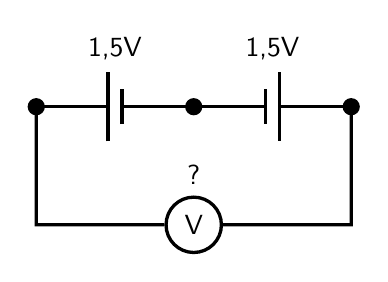
\begin{tikzpicture}[circuit ee IEC,y=1.5cm,x=2cm]
  \node [contact] (left) at (0,1) {};
  \node [contact] (middle) at (1,1) {};
  \node [contact] (right) at (2,1) {};
  \draw (left) to [battery={info={1,5V}}] (middle);
  \draw (right) to [battery={info'={1,5V}}] (middle);
  \draw (0,1) to (0,0) to [voltmeter={info={?}}] (2,0) to (2,1);
\end{tikzpicture}}
\answer{0 V}
\answer{3 V}
\answer{-3 V}
\answer{1,5 V}
\end{question}

\begin{question}{TB202}{Folgende Schaltung eines Akkus besteht aus Zellen von je 2 V. Jede Zelle kann 10 Ah Ladung liefern. Welche Daten hat der Akku?}
\answer{12 V / 10 Ah}
\answer{12 V / 60 Ah}
\answer{2 V / 10 Ah}
\answer{2 V / 60 Ah}
\end{question}

\begin{question}{TB203}{Was versteht man unter „technischer Stromrichtung“ in der Elektrotechnik?}
\answer{Man nimmt an, dass der Strom vom Pluspol zum Minuspol fließt.}
\answer{Man nimmt an, dass der Strom vom Minuspol zum Pluspol fließt.}
\answer{Es ist die Flussrichtung der Elektronen vom Minuspol zum Pluspol.}
\answer{Es ist die Flussrichtung der Elektronen vom Pluspol zum Minuspol.}
\end{question}

\begin{question}{TB204}{Kann in folgender Schaltung von zwei gleichen Spannungsquellen Strom fließen? Welche Begründung ist richtig?}
\answer{Nein, weil kein geschlossener Stromkreis vorhanden ist.}
\answer{Nein, weil der Pluspol mit dem Minuspol verbunden ist.}
\answer{Ja, sogar Kurzschlussstrom, weil der Pluspol mit dem Minuspol verbunden ist.}
\answer{Ja. Der Strom hängt vom Innenwiderstand der Batterien ab.}
\end{question}

\begin{question}{TB205}{Wie lange könnte man mit einem voll geladenen Akku mit 55 Ah einen Amateurfunkempfänger betreiben, der einen Strom von 0,8 A aufnimmt?}
\answer{68 Stunden und 45 Minuten}
\answer{Genau 44 Stunden}
\answer{6 Stunden 52 Minuten und 30 Sekunden}
\answer{69 Stunden und 15 Minuten}
\end{question}

\subsection{Elektrisches Feld}

\begin{question}{TB301}{Welche Einheit wird für die elektrische Feldstärke verwendet?}
\answer{Volt pro Meter (V/m)}
\answer{Watt pro Quadratmeter (W/m2)}
\answer{Ampere pro Meter (A/m)}
\answer{Henry pro Meter (H/m)}
\end{question}

\begin{question}{TB302}{Wie nennt man das Feld zwischen zwei parallelen Kondensatorplatten bei Anschluss einer Gleichspannung?}
\answer{Homogenes elektrisches Feld}
\answer{Homogenes magnetisches Feld}
\answer{Polarisiertes elektrisches Feld}
\answer{Polarisiertes magnetisches Feld}
\end{question}

\begin{question}{TB303}{Wie werden die mit X gekennzeichneten Feldlinien einer Vertikalantenne bezeichnet?}
\answer{Elektrische Feldlinien}
\answer{Magnetische Feldlinien}
\answer{Polarisierte Feldlinien}
\answer{Horizontale Feldlinien}
\end{question}

\subsection{Magnetisches Feld}

\begin{question}{TB401}{Welche Einheit wird für die magnetische Feldstärke verwendet?}
\answer{Ampere pro Meter (A/m)}
\answer{Watt pro Quadratmeter (W/m2)}
\answer{Volt pro Meter (V/m)}
\answer{Henry pro Meter (H/m)}
\end{question}

\begin{question}{TB402}{Wie nennt man das Feld im Innern einer langen Zylinderspule beim Fließen eines Gleichstroms?}
\answer{Homogenes magnetisches Feld}
\answer{Homogenes elektrisches Feld}
\answer{Konzentrisches magnetisches Feld}
\answer{Zentriertes magnetisches Feld}
\end{question}

\begin{question}{TB403}{Wenn Strom durch einen gestreckten Leiter fließt, entsteht ein}
\answer{Magnetfeld aus konzentrischen Kreisen um den Leiter.}
\answer{elektrisches Feld aus konzentrischen Kreisen um den Leiter.}
\answer{homogenes Magnetfeld um den Leiter.}
\answer{homogenes elektrisches Feld um den Leiter.}
\end{question}

\begin{question}{TB404}{Wie werden die mit X gekennzeichneten Feldlinien einer Vertikalantenne bezeichnet?}
\answer{Magnetische Feldlinien}
\answer{Elektrische Feldlinien}
\answer{Radiale Feldlinien}
\answer{Vertikale Feldlinien}
\end{question}

\begin{question}{TB405}{Welcher der nachfolgenden Werkstoffe ist ein ferromagnetischer Stoff?}
\answer{Eisen}
\answer{Chrom}
\answer{Kupfer}
\answer{Aluminium}
\end{question}

\subsection{Elektromagnetisches Feld}

\begin{question}{TB501}{Wodurch entsteht ein elektromagnetisches Feld? Ein elektromagnetisches Feld entsteht,}
\answer{wenn ein zeitlich schnell veränderlicher Strom durch einen elektrischen Leiter fließt, dessen Länge mindestens 1/100 der Wellenlänge ist.}
\answer{wenn durch einen elektrischen Leiter, dessen Länge mindestens 1/100 der Wellenlänge ist, ein konstanter Strom fließt.}
\answer{wenn sich elektrische Ladungen in einem Leiter befinden, dessen Länge mindestens 1/100 der Wellenlänge ist.}
\answer{wenn an einem elektrischen Leiter, dessen Länge mindestens 1/100 der Wellenlänge ist, eine konstante Spannung angelegt wird.}
\end{question}

\begin{question}{TB502}{Wie erfolgt die Ausbreitung einer elektromagnetischen Welle? Die Ausbreitung erfolgt}
\answer{durch eine Wechselwirkung zwischen elektrischem und magnetischem Feld.}
\answer{nur über das elektrische Feld. Das magnetische Feld ist nur im Nahfeld vorhanden.}
\answer{nur über das magnetische Feld. Das elektrische Feld ist nur im Nahfeld vorhanden.}
\answer{über die sich unabhängig voneinander ausbreitenden und senkrecht zueinander stehenden elektrischen und magnetischen Felder.}
\end{question}

\begin{question}{TB503}{Das folgende Bild zeigt die Feldlinien eines elektromagnetischen Feldes. Welche Polari sation hat die skizzierte Wellenfront?}
\answer{Horizontale Polarisation}
\answer{Vertikale Polarisation}
\answer{Rechtsdrehende Polarisation}
\answer{Zirkulare Polarisation}
\end{question}

\begin{question}{TB504}{Der Winkel zwischen den elektrischen und magnetischen Feldkomponenten eines elektromagnetischen Feldes beträgt im Fernfeld}
\answer{90°.}
\answer{45°.}
\answer{180°.}
\answer{360°.}
\end{question}

\begin{question}{TB505}{Die Polarisation des Sendesignals in der Hauptstrahlrichtung dieser Richtantenne ist}
\answer{vertikal.}
\answer{horizontal.}
\answer{rechtsdrehend.}
\answer{linksdrehend.}
\end{question}

\subsection{Sinusförmige Signale}

\begin{question}{TB601}{Welches ist die Einheit der Wellenlänge?}
\answer{m}
\answer{m/s}
\answer{Hz}
\answer{s/m}
\end{question}

\begin{question}{TB602}{Welcher Wellenlänge λ entspricht die Frequenz 1,84 MHz?}
\answer{163 m}
\answer{16,3 m}
\answer{10,5 m}
\answer{61,3 m}
\end{question}

\begin{question}{TB603}{Welcher Wellenlänge λ entspricht die Frequenz 28,48 MHz?}
\answer{10,5 m}
\answer{163 m}
\answer{9,49 m}
\answer{61,3 m}
\end{question}

\begin{question}{TB604}{Eine Wellenlänge von 2,06 m entspricht einer Frequenz von}
\answer{145,631 MHz}
\answer{148,927 MHz}
\answer{150,247 MHz}
\answer{135,754 MHz}
\end{question}

\begin{question}{TB605}{Eine Wellenlänge von 80,0 m entspricht einer Frequenz von}
\answer{3,75 MHz}
\answer{3,65 MHz}
\answer{3,56 MHz}
\answer{3,57 MHz}
\end{question}

\begin{question}{TB606}{Welche Bezeichnung ist für eine Schwingung von 145 000 000 Perioden pro Sekunde richtig?}
\answer{145 MHz}
\answer{145 μs}
\answer{145 kHz}
\answer{145 km/s}
\end{question}

\begin{question}{TB607}{Die Periodendauer von 50 μs entspricht einer Frequenz von}
\answer{20 kHz}
\answer{2 MHz}
\answer{200 kHz}
\answer{20 MHz}
\end{question}

\begin{question}{TB608}{Den Frequenzbereich zwischen 30 und 300 MHz bezeichnet man als}
\answer{VHF (very high frequency)}
\answer{UHF (ultra high frequency)}
\answer{MF (medium frequency)}
\answer{SHF (super high frequency)}
\end{question}

\begin{question}{TB609}{Das 70-cm-Band befindet sich im}
\answer{UHF-Bereich.}
\answer{VHF-Bereich.}
\answer{SHF-Bereich.}
\answer{EHF-Bereich.}
\end{question}

\begin{question}{TB610}{Welche Frequenz hat die in diesem Oszillogramm dargestellte Spannung?}
\answer{83,3 kHz}
\answer{833,3 kHz}
\answer{8,3 MHz}
\answer{83,3 MHz}
\end{question}

\begin{question}{TB611}{Welche Frequenz hat das in diesem Schirmbild dargestellte Signal?}
\answer{8,33 MHz}
\answer{16,7 MHz}
\answer{8,33 kHz}
\answer{833 kHz}
\end{question}

\begin{question}{TB612}{Eine sinusförmige Wechselspannung hat einen Spitzenwert von 12 V. Wie groß ist der Effektivwert der Wechselspannung?}
\answer{8,5 V}
\answer{6,0 V}
\answer{17 V}
\answer{24 V}
\end{question}

\begin{question}{TB613}{Ein sinusförmiges Signal hat einen Effektivwert von 12 V. Wie groß ist der Spitzen- Spitzen-Wert?}
\answer{33,9 V}
\answer{24 V}
\answer{16,97 V}
\answer{36,4 V}
\end{question}

\subsection{Nichtsinusförmige Signale}

\begin{question}{TB701}{Welche Signalform sollte der Träger einer hochfrequenten Schwingung haben?}
\answer{sinusförmig}
\answer{rechteckförmig}
\answer{dreieckförmig}
\answer{kreisförmig}
\end{question}

\begin{question}{TB702}{Ein periodische Schwingung, die wie das folgende Signal aussieht, besteht}
\answer{aus der Grundwelle mit ganzzahligen Vielfachen dieser Frequenz (Oberwellen).}
\answer{aus der Grundwelle und Teilen dieser Frequenz (Unterwellen).}
\answer{aus nur einer einzigen Frequenz.}
\answer{aus der Grundwelle mit vielen Nebenfrequenzen.}
\end{question}

\subsection{Modulierte Signale}

\begin{question}{TB801}{Was ist der Unterschied zwischen AM und SSB?}
\answer{AM hat einen Träger und zwei Seitenbänder, SSB arbeitet mit Trägerunterdrückung und einem Seitenband.}
\answer{AM hat einen Träger und ein Seitenband, SSB arbeitet mit Trägerunterdrückung und hat zwei Seitenbänder.}
\answer{AM hat keinen Träger und zwei Seitenbänder, SSB arbeitet mit Trägerunterdrückung und einem Seitenband.}
\answer{AM hat keinen Träger und zwei Seitenbänder, SSB arbeitet mit Träger und einem Seitenband.}
\end{question}

\begin{question}{TB802}{Was ist der Unterschied zwischen LSB und USB?}
\answer{LSB arbeitet mit Trägerunterdrückung und dem unteren Seitenband, USB arbeitet mit Trägerunterdrückung und dem oberen Seitenband.}
\answer{LSB arbeitet mit Träger und zwei Seitenbändern, USB arbeitet mit Trägerunterdrückung und einem Seitenband.}
\answer{LSB arbeitet mit Träger und einem Seitenband, USB arbeitet mit Trägerunterdrückung und beiden Seitenbändern.}
\answer{LSB arbeitet mit Trägerunterdrückung und dem oberen Seitenband, USB arbeitet mit Trägerunterdrückung und dem unteren Seitenband.}
\end{question}

\begin{question}{TB803}{Welche Aussage über modulierte Signale ist richtig?}
\answer{Bei FM ändert sich die Amplitude des Sendesignals bei Modulation nicht.}
\answer{Bei SSB ändert sich die Amplitude des Sendesignals bei Modulation nicht.}
\answer{Bei FM ändert sich die Amplitude des Sendesignals bei Modulation im Rhythmus der Sprache.}
\answer{Bei AM ändert sich die Amplitude des Sendesignals bei Modulation nicht.}
\end{question}

\begin{question}{TB804}{Was ist der Unterschied zwischen FSK und AFSK?}
\answer{Bei FSK wird der Träger direkt und bei AFSK mit Hilfe des Audiosignals moduliert.}
\answer{Bei FSK wird der Träger frequenzmoduliert und bei AFSK amplitudenmoduliert.}
\answer{Bei FSK wird der Träger frequenzmoduliert und bei AFSK wird der Träger unterdrückt.}
\answer{Bei FSK wird der Träger amplitudenmoduliert und bei AFSK frequenzmoduliert.}
\end{question}

\begin{question}{TB805}{Wie groß ist die HF-Bandbreite, die bei der Übertragung eines SSB-Signals entsteht?}
\answer{Sie entspricht genau der Bandbreite des NF- Signals.}
\answer{Sie entspricht der Hälfte der Bandbreite des NF-Signals.}
\answer{Sie entspricht der doppelten Bandbreite des NF-Signals.}
\answer{Sie ist Null, weil bei SSB-Modulation der HF- Träger unterdrückt wird.}
\end{question}

\begin{question}{TB806}{Ein Träger von 3,65 MHz wird mit der NF- Frequenz von 2 kHz in SSB (LSB) moduliert. Welche Frequenz/Frequenzen treten im modulierten HF-Signal hauptsächlich auf?}
\answer{3,648 MHz}
\answer{3,650 MHz}
\answer{3,652 MHz}
\answer{3,648 MHz und 3,652 MHz}
\end{question}

\subsection{Ohmsches Gesetz, Leistung und Energie}

\begin{question}{TB901}{Die Maßeinheit der elektrischen Leistung ist}
\answer{Watt}
\answer{Joule}
\answer{Kilowattstunden}
\answer{Amperestunden}
\end{question}

\begin{question}{TB902}{Welcher der nachfolgenden Zusammenhänge ist richtig?}
\answer{U = R ⋅ I}
\answer{I = U ⋅R}
\answer{IR = U}
\answer{RI = U}
\end{question}

\begin{question}{TB903}{Welche Spannung lässt einen Strom von 2 A durch einen Widerstand von 50 Ohm flie- ßen?}
\answer{100 Volt}
\answer{200 Volt}
\answer{25 Volt}
\answer{52 Volt}
\end{question}

\begin{question}{TB904}{Welcher Widerstand ist erforderlich um einen Strom von 3 A bei einer Spannung von 90 Volt fließen zu lassen?}
\answer{30 Ω}
\answer{1/30 Ω}
\answer{270 Ω}
\answer{93 Ω}
\end{question}

\begin{question}{TB905}{Eine Stromversorgung nimmt bei 230 V einen Strom von 0,63 A auf. Welche elektrische Arbeit (Energie) wird bei einer Betriebsdauer von 7 Stunden verbraucht?}
\answer{1,01 kWh}
\answer{0,1 kWh}
\answer{2,56 kWh}
\answer{20,7 kWh}
\end{question}

\begin{question}{TB906}{Eine Glühlampe hat einen Nennwert von 12 V und 48 W. Bei einer 12-V-Versorgung beträgt die Stromentnahme}
\answer{4 A.}
\answer{250 mA.}
\answer{750 mA.}
\answer{36 A.}
\end{question}

\begin{question}{TB907}{Der Effektivwert der Spannung an einer künstlichen 50-Ω-Antenne wird mit 100 V gemessen. Die Leistung an der Last beträgt}
\answer{200 W.}
\answer{141 W.}
\answer{100 W.}
\answer{283 W.}
\end{question}

\begin{question}{TB908}{Ein mit einer künstlichen 50-Ω-Antenne in Serie geschaltetes Amperemeter zeigt 2 A an. Die Leistung in der Last beträgt}
\answer{200 W.}
\answer{100 W.}
\answer{25 W.}
\answer{250 W.}
\end{question}

\begin{question}{TB909}{Ein Mobil-Transceiver (Sender-Empfänger) hat bei Sendebetrieb eine Leistungsaufnahme von 100 Watt aus dem 12-V-Bordnetz des Kraftfahrzeuges. Wie groß ist die Stromaufnahme?}
\answer{8,33 A}
\answer{16,6 A}
\answer{1200 A}
\answer{0,12 A}
\end{question}

\begin{question}{TB910}{Ein 100-Ω-Widerstand, an dem 10 V anliegen, muss mindestens eine Belastbarkeit haben von}
\answer{1 W.}
\answer{10 W.}
\answer{0,01 W.}
\answer{100 mW.}
\end{question}

\begin{question}{TB911}{Welche Belastbarkeit muss ein Vorwiderstand haben, an dem bei einem Strom von 50 mA eine Spannung von 50 V abfallen soll?}
\answer{2,5 W}
\answer{1 W}
\answer{25 W}
\answer{250 mW}
\end{question}

\section{Elektrische und elektronische Bauteile}

\subsection{Widerstand}

\begin{question}{TC101}{Die Farbringe gelb, violett und orange auf einem Widerstand mit 4 Farbringen bedeuten einen Widerstandswert von}
\answer{47 kΩ}
\answer{4,7 kΩ}
\answer{470 kΩ}
\answer{4,7 MΩ}
\end{question}

\begin{question}{TC102}{Die Farbringe gelb, violett und rot auf einem Widerstand mit 4 Farbringen bedeuten einen Widerstandswert von}
\answer{4,7 kΩ}
\answer{47 kΩ}
\answer{470 kΩ}
\answer{4,7 MΩ}
\end{question}

\begin{question}{TC103}{Die Farbringe rot, violett und orange auf einem Widerstand mit 4 Farbringen bedeuten einen Widerstandswert von}
\answer{27 kΩ}
\answer{2,7 kΩ}
\answer{270 kΩ}
\answer{2,7 MΩ}
\end{question}

\begin{question}{TC104}{Die Farbringe rot, violett und rot auf einem Widerstand mit 4 Farbringen bedeuten einen Widerstandswert von}
\answer{2,7 kΩ}
\answer{27 kΩ}
\answer{270 kΩ}
\answer{2,7 MΩ}
\end{question}

\begin{question}{TC105}{Welches Bauteil hat folgendes Schaltzeichen?}
\answer{NTC}
\answer{PTC}
\answer{LDR}
\answer{VDR}
\end{question}

\begin{question}{TC106}{Welches der folgenden Bauteile ist ein NTC?}
\answer{C}
\answer{D}
\end{question}

\begin{question}{TC107}{Welches der folgenden Schaltsymbole stellt einen PTC-Widerstand dar?}
\answer{C}
\answer{D}
\end{question}

\begin{question}{TC108}{Ein Widerstand hat eine Toleranz von 10 \%. Bei einem nominalen Widerstandswert von 5,6 kΩ liegt der tatsächliche Wert zwischen}
\answer{5040 und 6160 Ω.}
\answer{4760 und 6440 Ω.}
\answer{4,7 und 6,8 kΩ.}
\answer{5,2 und 6,3 kΩ.}
\end{question}

\begin{question}{TC109}{Welche Bauart von Widerstand folgender Auswahl ist am besten für eine künstliche Antenne (Dummy Load) geeignet?}
\answer{Ein Metalloxidwiderstand}
\answer{Ein Kohleschichtwiderstand}
\answer{Ein keramischer Drahtwiderstand}
\answer{Ein frei gewickelter Drahtwiderstand aus Kupferdraht}
\end{question}

\begin{question}{TC110}{Welchen Wert hat ein SMD-Widerstand mit der Kennzeichnung 221?}
\answer{220 Ω}
\answer{221 Ω}
\answer{22 Ω}
\answer{22 kΩ}
\end{question}

\begin{question}{TC111}{Welchen Wert hat ein SMD-Widerstand mit der Kennzeichnung 223?}
\answer{22 kΩ}
\answer{221 Ω}
\answer{22 Ω}
\answer{220 Ω}
\end{question}

\subsection{Kondensator}

\begin{question}{TC201}{Welche Aussage zur Kapazität eines Plattenkondensators ist richtig?}
\answer{Je größer der Plattenabstand ist, desto kleiner ist die Kapazität.}
\answer{Je größer die angelegte Spannung ist, desto kleiner ist die Kapazität.}
\answer{Je größer die Plattenoberfläche ist, desto kleiner ist die Kapazität.}
\answer{Je größer die Dielektrizitätszahl ist, desto kleiner ist die Kapazität.}
\end{question}

\begin{question}{TC202}{Ein Bauelement, bei dem sich Platten auf einer isolierten Achse befinden, die zwischen fest stehende Platten hineingedreht werden können, nennt man}
\answer{Drehkondensator.}
\answer{Tauchkondensator.}
\answer{Keramischer Kondensator.}
\answer{Rotorkondensator.}
\end{question}

\begin{question}{TC203}{Welche Kapazität hat nebenstehend abgebildeter Kondensator?}
\answer{330 μF}
\answer{3,3 μF}
\answer{33 μF}
\answer{33000 μF}
\end{question}

\begin{question}{TC204}{Welche Kapazität hat nebenstehend abgebildeter Kondensator?}
\answer{470 pF}
\answer{4,7 pF}
\answer{47 pF}
\answer{47000 pF}
\end{question}

\begin{question}{TC205}{Welche Kapazität hat nebenstehend abgebildeter Kondensator?}
\answer{8,2 pF}
\answer{820 pF}
\answer{82 pF}
\answer{0,82 pF}
\end{question}

\begin{question}{TC206}{Drei Kondensatoren mit den Kapazitäten C1 = 0,1 μF, C2 = 150 nF und C3 = 50000 pF werden parallel geschaltet. Wie groß ist die Gesamtkapazität?}
\answer{0,3 μF}
\answer{2,73 nF}
\answer{0,027 μF}
\answer{0,255 μF}
\end{question}

\begin{question}{TC207}{Bei welchem der folgenden Bauformen von Kondensatoren muss beim Einbau auf die Polarität geachtet werden?}
\answer{Elektrolytkondensator}
\answer{Keramischer Kondensator}
\answer{Styroflexkondensator}
\answer{Plattenkondensator}
\end{question}

\begin{question}{TC208}{Mit zunehmender Frequenz}
\answer{sinkt der Wechselstromwiderstand von Kondensatoren.}
\answer{sinkt der Wechselstromwiderstand von Kondensatoren bis zu einem Minimum und steigt dann wieder.}
\answer{steigt der Wechselstromwiderstand von Kondensatoren.}
\answer{steigt der Wechselstromwiderstand von Kondensatoren bis zu einem Maximum und sinkt dann wieder.}
\end{question}

\subsection{Spule}

\begin{question}{TC301}{Wie ändert sich die Induktivität einer Spule von 12 μH, wenn die Windungszahl bei gleicher Wickellänge verdoppelt wird?}
\answer{Die Induktivität steigt auf 48 μH.}
\answer{Die Induktivität steigt auf 24 μH.}
\answer{Die Induktivität sinkt auf 6 μH.}
\answer{Die Induktivität sinkt auf 3 μH.}
\end{question}

\begin{question}{TC302}{Wie ändert sich die Induktivität einer Spule von 12 μH, wenn die Wicklung auf dem Wickelkörper bei gleicher Windungszahl auf die doppelte Länge auseinander gezogen wird?}
\answer{Die Induktivität sinkt auf 6 μH.}
\answer{Die Induktivität steigt auf 24 μH.}
\answer{Die Induktivität steigt auf 48 μH.}
\answer{Die Induktivität sinkt auf 3 μH.}
\end{question}

\begin{question}{TC303}{Wie kann man die Induktivität einer Spule vergrößern?}
\answer{Durch Stauchen der Spule (Verkürzen der Spulenlänge).}
\answer{Durch Auseinanderziehen der Spule (Vergrößerung der Spulenlänge).}
\answer{Durch Einführen eines Kupferkerns in die Spule.}
\answer{Durch Einbau der Spule in einen Abschirmbecher.}
\end{question}

\begin{question}{TC304}{Das folgende Bild zeigt einen Kern, um den ein Kabel für den Bau einer Netzdrossel gewickelt ist. Der Kern sollte aus}
\answer{Ferrit bestehen.}
\answer{Kunststoff bestehen.}
\answer{Stahl bestehen.}
\answer{aus gut leitendem Material bestehen.}
\end{question}

\begin{question}{TC305}{Schaltet man zwei Glühlampen gleichzeitig an eine Spannungsquelle, wobei eine Glühlampe zum Helligkeitsausgleich über einen Widerstand und die andere über eine Spule mit vielen Windungen und Eisenkern angeschlossen ist, so}
\answer{leuchtet H1 zuerst.}
\answer{leuchtet H2 zuerst.}
\answer{leuchten H1 und H2 genau gleich schnell.}
\answer{leuchtet H2 kurz auf und geht wieder aus. H1 leuchtet.}
\end{question}

\begin{question}{TC306}{Mit zunehmender Frequenz}
\answer{steigt der Wechselstromwiderstand einer Spule.}
\answer{sinkt der Wechselstromwiderstand einer Spule.}
\answer{sinkt der Wechselstromwiderstand einer Spule bis zu einem Minimum und steigt dann wieder.}
\answer{steigt der Wechselstromwiderstand einer Spule bis zu einem Maximum und sinkt dann wieder.}
\end{question}

\subsection{Übertrager und Transformatoren}

\begin{question}{TC401}{Ein Trafo liegt an 230 Volt und gibt 11,5 Volt ab. Seine Primärwicklung hat 600 Windungen. Wie groß ist seine Sekundärwindungszahl?}
\answer{30 Windungen}
\answer{20 Windungen}
\answer{52 Windungen}
\answer{180 Windungen}
\end{question}

\begin{question}{TC402}{Ein Trafo liegt an 45 Volt und gibt 180 Volt ab. Seine Primärwicklung hat 150 Windungen. Wie groß ist seine Sekundärwindungszahl?}
\answer{600 Windungen}
\answer{850 Windungen}
\answer{46 Windungen}
\answer{30 Windungen}
\end{question}

\begin{question}{TC403}{Die Primärspule eines Übertragers hat die fünffache Anzahl von Windungen der Sekundärspule. Wie hoch ist die erwartete Sekundärspannung, wenn die Primärspule an eine 230-V-Stromversorgung angeschlossen wird?}
\answer{46 Volt}
\answer{9,2 Volt}
\answer{23 Volt}
\answer{1150 Volt}
\end{question}

\subsection{Diode}

\begin{question}{TC501}{P-dotiertes Halbleitermaterial ist solches, das mit einem zusätzlichen Stoff versehen wurde, der}
\answer{weniger als vier Valenzelektronen enthält.}
\answer{mehr als vier Valenzelektronen enthält.}
\answer{genau vier Valenzelektronen enthält.}
\answer{keine Valenzelektronen enthält.}
\end{question}

\begin{question}{TC502}{N-leitendes Halbleitermaterial ist gekennzeichnet durch}
\answer{Überschuss an freien Elektronen.}
\answer{das Fehlen von Dotierungsatomen.}
\answer{das Fehlen von Atomen im Gitter des Halbleiterkristalls.}
\answer{bewegliche Elektronenlücken.}
\end{question}

\begin{question}{TC503}{Ein in Durchlassrichtung betriebener PN- Übergang ermöglicht}
\answer{den Stromfluss von P nach N.}
\answer{den Stromfluss von N nach P.}
\answer{keinen Stromfluss.}
\answer{den Elektronenfluss von P nach N.}
\end{question}

\begin{question}{TC504}{Eine in Sperrrichtung betriebene Diode hat}
\answer{einen hohen Widerstand.}
\answer{eine hohe Kapazität.}
\answer{eine geringe Impedanz.}
\answer{eine hohe Induktivität.}
\end{question}

\begin{question}{TC505}{Die Auswahlantworten enthalten Silizium- Dioden mit unterschiedlichen Arbeitspunkten. Bei welcher Antwort befindet sich die Diode in leitendem Zustand?}
\answer{0,7 V 1,3 V}
\answer{-2,6 V -2,0 V}
\answer{15 V 9 V}
\answer{3,4 V 4,0 V}
\end{question}

\begin{question}{TC506}{Die Auswahlantworten enthalten Silizium- Dioden mit unterschiedlichen Arbeitspunkten. Bei welcher Antwort befindet sich die Diode in leitendem Zustand?}
\answer{-2 V -2,6 V}
\answer{5,3 V 4,7 V}
\answer{15 V 18 V}
\answer{3,9 V 3,2 V}
\end{question}

\begin{question}{TC507}{Wie verhält sich die Kapazität einer Kapazitätsdiode (Varicap)?}
\answer{Sie nimmt mit abnehmender Sperrspannung zu.}
\answer{Sie erhöht sich mit zunehmender Durchlassspannung.}
\answer{Sie nimmt mit zunehmender Sperrspannung zu.}
\answer{Sie erhöht sich mit zunehmendem Durchlassstrom.}
\end{question}

\begin{question}{TC508}{Wozu dient folgende Schaltung? Sie dient}
\answer{zur Spannungsstabilisierung.}
\answer{zur Signalbegrenzung.}
\answer{als Leuchtanzeige.}
\answer{zur Stromgewinnung.}
\end{question}

\begin{question}{TC509}{Wozu dient die folgende Schaltung? Sie dient}
\answer{als Leuchtanzeige.}
\answer{zur Signalbegrenzung.}
\answer{zur Spannungsstabilisierung.}
\answer{zur Stromgewinnung.}
\end{question}

\subsection{Transistor}

\begin{question}{TC601}{Was versteht man unter Stromverstärkung beim Transistor?}
\answer{Mit einem geringen Strom (Basisstrom) wird ein großer Strom (Kollektorstrom) gesteuert.}
\answer{Mit einem geringen Strom (Emitterstrom) wird ein großer Strom (Kollektorstrom) gesteuert.}
\answer{Mit einem geringen Strom (Emitterstrom) wird ein großer Strom (Basisstrom) gesteuert.}
\answer{Mit einem geringen Strom (Kollektorstrom) wird ein großer Strom (Emitterstrom) gesteuert.}
\end{question}

\begin{question}{TC602}{Das Verhältnis von Kollektorstrom zum Basisstrom eines Transistors liegt üblicherweise im Bereich von}
\answer{10 zu 1  bis  900 zu 1.}
\answer{1 zu 50  bis 1 zu 100.}
\answer{1000 zu 1  bis  5000 zu 1.}
\answer{1 zu 100  bis 1 zu 500.}
\end{question}

\begin{question}{TC603}{Bei diesem Bauelement handelt es sich um einen}
\answer{NPN-Transistor.}
\answer{PNP-Transistor.}
\answer{Sperrschicht-FET.}
\answer{MOSFET.}
\end{question}

\begin{question}{TC604}{Bei diesem Bauelement handelt es sich um einen}
\answer{PNP-Transistor.}
\answer{NPN-Transistor.}
\answer{P-Kanal-FET.}
\answer{N-Kanal-FET.}
\end{question}

\begin{question}{TC605}{Welche Kollektorspannungen haben NPNund PNP-Transistoren?}
\answer{NPN-Transistoren benötigen positive, PNP- Transistoren negative Kollektorspannungen.}
\answer{NPN- und PNP-Transistoren benötigen negative Kollektorspannungen.}
\answer{PNP-Transistoren benötigen positive, NPN- Transistoren negative Kollektorspannung.}
\answer{PNP- und NPN-Transistoren benötigen positive Kollektorspannungen.}
\end{question}

\begin{question}{TC606}{Bei einem bipolaren Transistor in leitendem Zustand befindet sich die Emitter-Basis- Diode}
\answer{in Durchlassrichtung.}
\answer{im Leerlauf.}
\answer{im Kurzschluss.}
\answer{in Sperrrichtung.}
\end{question}

\begin{question}{TC607}{Welche Transistortypen sind bipolare Transistoren?}
\answer{NPN- und PNP-Transistoren}
\answer{Dual-Gate-MOS-FETs}
\answer{Isolierschicht-FETs}
\answer{Sperrschicht-FETs}
\end{question}

\begin{question}{TC608}{Wie lauten die Bezeichnungen der Anschlüsse eines bipolaren Transistors?}
\answer{Emitter, Basis, Kollektor}
\answer{Emitter, Drain, Source}
\answer{Drain, Source, Kollektor}
\answer{Drain, Gate, Source}
\end{question}

\begin{question}{TC609}{Ein bipolarer Transistor ist}
\answer{stromgesteuert.}
\answer{spannungsgesteuert.}
\answer{thermisch gesteuert.}
\answer{ein Gleichspannungsverstärker.}
\end{question}

\begin{question}{TC610}{Wenn die Basisspannung eines NPN- Transistors gleich der Emitterspannung ist,}
\answer{fließt kein Kollektorstrom.}
\answer{fließt ein Kollektorstrom von etwa 0,6 A.}
\answer{liegt der Kollektorstrom zwischen 10 mA und 2 A.}
\answer{fließt ein sehr hoher Kollektor-Kurzschlussstrom.}
\end{question}

\begin{question}{TC611}{Wie erfolgt die Steuerung des Stroms im Feldeffekttransistor (FET)?}
\answer{Die Gatespannung steuert den Widerstand des Kanals zwischen Source und Drain.}
\answer{Die Gatespannung ist allein verantwortlich für den Drainstrom.}
\answer{Der Gatestrom ist allein verantwortlich für den Drainstrom.}
\answer{Der Gatestrom steuert den Widerstand des Kanals zwischen Source und Drain.}
\end{question}

\begin{question}{TC612}{Wie bezeichnet man die Anschlüsse des nebenstehenden Transistors?}
\answer{1 ... Drain, 2 ... Source,}
\answer{1 ... Source, 2 ... Drain,}
\answer{1 ... Anode, 2 ... Katode,}
\answer{1 ... Kollektor, 2 ... Emitter,}
\end{question}

\section{Elektronische Schaltungen und deren Merkmale}

\subsection{Serien- und Parallelschaltung von Widerständen, Spulen und Kondensatoren}

\begin{question}{TD101}{Wie groß ist der Ersatzwiderstand der Gesamtschaltung? Gegeben: R1 = 500 Ω,  R2 = 1000 Ω und R3 = 1 kΩ}
\answer{1 kΩ}
\answer{2,5 kΩ}
\answer{501 Ω}
\answer{5,1 kΩ}
\end{question}

\begin{question}{TD102}{Wie groß ist der Ersatzwiderstand der Gesamtschaltung? Gegeben: R1 = 1 kΩ,  R2 = 2000 Ω und R3 = 2 kΩ}
\answer{2 kΩ}
\answer{2,5 kΩ}
\answer{501 Ω}
\answer{5,1 kΩ}
\end{question}

\begin{question}{TD103}{Wie groß ist der Ersatzwiderstand der Gesamtschaltung? Gegeben: R1 = 500 Ω,  R2 = 500 Ω und R3 = 1 kΩ}
\answer{500 Ω}
\answer{250 Ω}
\answer{1 kΩ}
\answer{2 kΩ}
\end{question}

\begin{question}{TD104}{Wie groß ist der Ersatzwiderstand der Gesamtschaltung? Gegeben: R1 = 500 Ω,  R2 = 1,5 kΩ und R3 = 2 kΩ}
\answer{1 kΩ}
\answer{4 kΩ}
\answer{500 Ω}
\answer{2 kΩ}
\end{question}

\begin{question}{TD105}{Welche Gesamtkapazität hat die folgende Schaltung? Gegeben: C1 = 0,01 μF;  C2 = 5 nF,  C3 = 5000 pF}
\answer{5 nF}
\answer{0,015 nF}
\answer{7,5 nF}
\answer{10 nF}
\end{question}

\begin{question}{TD106}{Welche Gesamtkapazität hat die folgende Schaltung? Gegeben: C1 = 0,02 μF; C2 = 10 nF; C3 = 10000 pF}
\answer{10 nF}
\answer{5 nF}
\answer{2,5 nF}
\answer{40 nF}
\end{question}

\begin{question}{TD107}{Welche Gesamtkapazität hat die folgende Schaltung? Gegeben: C1 = 0,01 μF; C2 = 10 nF; C3 = 5000 pF}
\answer{10 nF}
\answer{5 nF}
\answer{2,5 nF}
\answer{0,015 nF}
\end{question}

\begin{question}{TD108}{Die Gesamtspannung U an folgendem Spannungsteiler beträgt 12,2 V. Die Widerstände haben die Werte R1 = 10 kΩ und R2 = 2,2 kΩ. Wie groß ist die Teilspannung U2?}
\answer{2,20 V}
\answer{2,64 V}
\answer{10,0 V}
\answer{1,22 V}
\end{question}

\begin{question}{TD109}{Zwei Widerstände mit R1 = 20 Ω und R2 = 30 Ω sind parallel geschaltet. Wie groß ist der Ersatzwiderstand?}
\answer{12 Ω}
\answer{50 Ω}
\answer{15 Ω}
\answer{3,5 Ω}
\end{question}

\begin{question}{TD110}{Zwei Widerstände mit R1 = 100 Ω und R2 = 150 Ω sind parallel geschaltet. Wie groß ist der Ersatzwiderstand?}
\answer{60 Ω}
\answer{250 Ω}
\answer{75 Ω}
\answer{17,5 Ω}
\end{question}

\subsection{Schwingkreise und Filter}

\begin{question}{TD201}{Der Impedanzfrequenzgang in der Abbildung zeigt die Kennlinie}
\answer{eines Serienschwingkreises.}
\answer{eines Parallelschwingkreises.}
\answer{einer Induktivität.}
\answer{einer Kapazität.}
\end{question}

\begin{question}{TD202}{Der im folgenden Bild dargestellte Impedanzfrequenzgang ist typisch für}
\answer{einen Parallelschwingkreis.}
\answer{einen Kondensator.}
\answer{eine Spule.}
\answer{einen Serienschwingkreis.}
\end{question}

\begin{question}{TD203}{Welcher Schwingkreis passt zu dem neben der jeweiligen Schaltung dargestellten Verlauf des Scheinwiderstandes?}
\answer{}
\answer{}
\answer{}
\answer{}
\end{question}

\begin{question}{TD204}{Wie ändert sich die Resonanzfrequenz eines Schwingkreises, wenn 1. die Spule weniger Windungen erhält, 2. die Länge der Spule durch Zusammenschieben der Drahtwicklung verringert wird, 3. ein Ferritkern in das Innere der Spule gebracht wird?}
\answer{Die Resonanzfrequenz wird bei 1. größer und bei 2. und 3. kleiner.}
\answer{Die Resonanzfrequenz wird bei 1. und 2. kleiner und bei 3. größer.}
\answer{Die Resonanzfrequenz wird bei 1. kleiner und bei 2. und 3. größer.}
\answer{Die Resonanzfrequenz wird bei 1. und 2. grö- ßer und bei 3. kleiner.}
\end{question}

\begin{question}{TD205}{Wie verhält sich ein Parallelschwingkreis bei der Resonanzfrequenz?}
\answer{Wie ein hochohmiger Widerstand.}
\answer{Wie ein niederohmiger Widerstand.}
\answer{Wie ein Kondensator mit sehr kleiner Kapazität.}
\answer{Wie eine Spule mit sehr großer Induktivität.}
\end{question}

\begin{question}{TD206}{Was stellt die folgende Schaltung dar?}
\answer{Hochpass}
\answer{Sperrkreis}
\answer{Bandpass}
\answer{Tiefpass}
\end{question}

\begin{question}{TD207}{Was stellt die folgende Schaltung dar?}
\answer{Sperrkreis}
\answer{Saugkreis}
\answer{Bandpass}
\answer{Tiefpass}
\end{question}

\begin{question}{TD208}{Was stellt die folgende Schaltung dar?}
\answer{Tiefpass}
\answer{Sperrkreis}
\answer{Bandpass}
\answer{Hochpass}
\end{question}

\begin{question}{TD209}{Was stellt die folgende Schaltung dar?}
\answer{Saugkreis}
\answer{Sperrkreis}
\answer{Bandpass}
\answer{Tiefpass}
\end{question}

\begin{question}{TD210}{Welche der nachfolgenden Eigenschaften trifft auf einen Hochpass zu?}
\answer{Frequenzen oberhalb der Grenzfrequenz werden durchgelassen.}
\answer{Frequenzen unterhalb der Grenzfrequenz werden verstärkt.}
\answer{Frequenzen oberhalb der Grenzfrequenz werden stark bedämpft.}
\answer{Frequenzen unterhalb der Grenzfrequenz werden ungedämpft durchgelassen.}
\end{question}

\subsection{Stromversorgung}

\begin{question}{TD301}{Welche Eigenschaften sollten Strom- und Spannungsquellen aufweisen?}
\answer{Spannungsquellen sollten einen möglichst niedrigen Innenwiderstand und Stromquellen einen möglichst hohen Innenwiderstand haben.}
\answer{Strom- und Spannungsquellen sollten einen möglichst niedrigen Innenwiderstand haben.}
\answer{Strom- und Spannungsquellen sollten einen möglichst hohen Innenwiderstand haben.}
\answer{Spannungsquellen sollten einen möglichst hohen Innenwiderstand und Stromquellen einen möglichst niedrigen Innenwiderstand haben.}
\end{question}

\begin{question}{TD302}{Die Leerlaufspannung einer Gleichspannungsquelle beträgt 13,5 V. Wenn die Spannungsquelle einen Strom von 1 A abgibt, sinkt die Klemmenspannung auf 12,4 V. Wie groß ist der Innenwiderstand der Spannungsquelle?}
\answer{1,1 Ω}
\answer{13,5 Ω}
\answer{12,4 Ω}
\answer{1,2 Ω}
\end{question}

\begin{question}{TD303}{Die Leerlaufspannung einer Gleichspannungsquelle beträgt 13,5 V. Wenn die Spannungsquelle einen Strom von 2 A abgibt, sinkt die Klemmenspannung auf 13 V. Wie groß ist der Innenwiderstand der Spannungsquelle?}
\answer{0,25 Ω}
\answer{6,75 Ω}
\answer{13 Ω}
\answer{6,5 Ω}
\end{question}

\begin{question}{TD304}{Berechnen Sie die Leerlaufausgangsspannung dieser Schaltung für ein Transformationsverhältnis von 5:1.}
\answer{Zirka 65 Volt}
\answer{Zirka 46 Volt}
\answer{Zirka 40 Volt}
\answer{Zirka 28 Volt}
\end{question}

\begin{question}{TD305}{Berechnen Sie die Leerlaufausgangsspannung dieser Schaltung für ein Transformationsverhältnis von 8:1.}
\answer{Zirka 40 Volt}
\answer{Zirka 46 Volt}
\answer{Zirka 65 Volt}
\answer{Zirka 28 Volt}
\end{question}

\begin{question}{TD306}{Welches ist der Hauptnachteil eines Schaltnetzteils gegenüber einem konventionellen Netzteil?}
\answer{Ein Schaltnetzteil erzeugt Oberwellen seiner Taktfrequenz, die beim Empfang zu Störungen führen können.}
\answer{Ein Schaltnetzteil benötigt einen größeren Transformator.}
\answer{Ein Schaltnetzteil kann keine so hohen Ströme abgeben.}
\answer{Ein Schaltnetzteil hat höhere Verluste.}
\end{question}

\subsection{Verstärker}

\begin{question}{TD401}{In welcher der folgenden Zeilen werden nur Verstärker-Bauelemente genannt?}
\answer{Transistor, MOSFET, Operationsverstärker, Röhre}
\answer{Transistor, Halbleiterdiode, Operationsverstärker, Röhre}
\answer{Transistor, Varicap-Diode, Operationsverstärker, Röhre}
\answer{Transistor, MOSFET, Halbleiterdiode, Röhre}
\end{question}

\begin{question}{TD402}{Was versteht man in der Elektronik unter Verstärkung? Man spricht von Verstärkung, wenn}
\answer{das Ausgangssignal gegenüber dem Eingangssignal in der Leistung größer ist.}
\answer{das Eingangssignal gegenüber dem Ausgangssignal in der Leistung größer ist.}
\answer{z.B. bei einem Transformator die Ausgangsspannung größer ist als die Eingangsspannung.}
\answer{das Eingangssignal gegenüber dem Ausgangssignal in der Spannung größer ist.}
\end{question}

\begin{question}{TD403}{Was ist ein Operationsverstärker?}
\answer{Operationsverstärker sind Gleichstrom gekoppelte Verstärker mit sehr hohem Verstärkungsfaktor und großer Linearität.}
\answer{Operationsverstärker sind Wechselstrom gekoppelte Verstärker mit niedrigem Eingangswiderstand und großer Linearität.}
\answer{Operationsverstärker sind in Empfängerstufen eingebaute Analogverstärker mit sehr niedrigem Verstärkungsfaktor aber großer Linearität.}
\answer{Operationsverstärker sind digitale Schaltkreise mit hohem Verstärkungsfaktor.}
\end{question}

\begin{question}{TD404}{Ein IC (integrated circuit) ist}
\answer{eine komplexe Schaltung auf einem Halbleiterkristallplättchen.}
\answer{eine aus vielen einzelnen Bauteilen aufgebaute Schaltung auf einer Platine.}
\answer{eine miniaturisierte, aus SMD-Bauteilen aufgebaute Schaltung.}
\answer{eine Zusammenschaltung verschiedener Baugruppen zu einer Funktionseinheit.}
\end{question}

\begin{question}{TD405}{Worauf beruht die Verstärkerwirkung von Elektronenröhren?}
\answer{Das von der Gitterspannung hervorgerufene elektrische Feld steuert den Anodenstrom.}
\answer{Die Anodenspannung steuert das magnetische Feld an der Anode und damit den Anodenstrom.}
\answer{Die Heizspannung steuert das elektrische Feld an der Kathode und damit den Anodenstrom.}
\answer{Die Katodenvorspannung steuert das magnetische Feld an der Kathode und damit den Gitterstrom.}
\end{question}

\subsection{Modulator / Demodulator}

\begin{question}{TD501}{Durch Modulation}
\answer{werden Informationen auf einen oder mehrere Träger übertragen.}
\answer{wird einem oder mehreren Trägern Informationen entnommen.}
\answer{werden Sprach- und CW-Signale kombiniert.}
\answer{werden dem Signal NF-Komponenten entnommen.}
\end{question}

\begin{question}{TD502}{Welche Aussage zum Frequenzmodulator ist richtig? Durch das Informationssignal}
\answer{wird die Frequenz des Trägers beeinflusst. Die Amplitude des Trägers bleibt dabei konstant.}
\answer{wird die Amplitude des Trägers beeinflusst. Die Frequenz des Trägers bleibt dabei konstant.}
\answer{werden gleichzeitig Frequenz und Amplitude des Trägers beeinflusst.}
\answer{findet keinerlei Beeinflussung von Trägerfrequenz oder Trägeramplitude statt. Die Information steuert nur die Kapazität des Oszillators.}
\end{question}

\begin{question}{TD503}{Zur Aufbereitung des SSB-Signals müssen}
\answer{der Träger und ein Seitenband unterdrückt oder ausgefiltert werden.}
\answer{der Träger hinzugesetzt und ein Seitenband ausgefiltert werden.}
\answer{der Träger unterdrückt und ein Seitenband hinzugesetzt werden.}
\answer{der Träger unterdrückt und beide Seitenbänder ausgefiltert werden.}
\end{question}

\begin{question}{TD504}{Wie kann ein SSB-Signal erzeugt werden?}
\answer{Im Balancemodulator wird ein Zweiseitenband- Signal erzeugt. Das Seitenbandfilter selektiert ein Seitenband heraus.}
\answer{Im Balancemodulator wird ein Zweiseitenband- Signal erzeugt. Ein auf die Trägerfrequenz abgestimmter Saugkreis filtert den Träger aus.}
\answer{Im Balancemodulator wird ein Einseitenband- Signal erzeugt. Ein auf die Trägerfrequenz abgestimmter Sperrkreis filtert den Träger aus.}
\answer{Im Balancemodulator wird ein Zweiseitenband- Signal erzeugt. In einem Frequenzteiler wird ein Seitenband abgespalten.}
\end{question}

\subsection{Oszillator}

\begin{question}{TD601}{Was verstehen Sie unter einem „Oszillator“?}
\answer{Es ist ein Schwingungserzeuger.}
\answer{Es ist ein sehr schmales Filter.}
\answer{Es ist ein Messgerät zur Anzeige von Schwingungen.}
\answer{Es ist ein FM-Modulator.}
\end{question}

\begin{question}{TD602}{Was ist ein LC-Oszillator? Es ist ein Schwingungserzeuger, wobei die Frequenz}
\answer{von einer Spule und einem Kondensator (LC- Schwingkreis) bestimmt wird.}
\answer{durch einen hochstabilen Quarz bestimmt wird.}
\answer{mittels LC-Tiefpass gefiltert wird.}
\answer{mittels LC-Hochpass gefiltert wird.}
\end{question}

\begin{question}{TD603}{Was ist ein Quarz-Oszillator? Es ist ein Schwingungserzeuger, wobei die Frequenz}
\answer{durch einen hochstabilen Quarz bestimmt wird.}
\answer{allein durch einen Quarz erzeugt wird.}
\answer{mittels Quarz-Tiefpass gefiltert wird.}
\answer{mittels Quarz-Hochpass gefiltert wird.}
\end{question}

\begin{question}{TD604}{Wie verhält sich die Frequenz eines LC- Oszillators bei Temperaturanstieg, wenn die Kapazität des Schwingkreiskondensators mit dem Temperaturanstieg geringer wird?}
\answer{Die Frequenz wird erhöht.}
\answer{Die Schwingungen reißen ab (Aussetzer).}
\answer{Die Frequenz wird niedriger.}
\answer{Die Frequenz bleibt stabil.}
\end{question}

\begin{question}{TD605}{Im VFO eines Senders steigt die Induktivität der Oszillatorspule mit der Temperatur. Der Kondensator bleibt sehr stabil. Welche Auswirkungen hat dies bei steigender Temperatur?}
\answer{Die VFO-Frequenz wandert nach unten.}
\answer{Die VFO-Frequenz wandert nach oben.}
\answer{Die VFO-Ausgangsspannung nimmt zu.}
\answer{Die VFO-Ausgangsspannung nimmt ab.}
\end{question}

\begin{question}{TD606}{Der Vorteil von Quarzoszillatoren gegenüber LC-Oszillatoren liegt darin, dass sie}
\answer{eine bessere Frequenzstabilität aufweisen.}
\answer{eine breitere Resonanzkurve haben.}
\answer{einen geringeren Anteil an Oberwellen erzeugen.}
\answer{ein sehr viel geringes Seitenbandrauschen erzeugen.}
\end{question}

\section{Analoge und digitale Modulationsverfahren}

\subsection{Amplitudenmodulation AM, SSB}

\begin{question}{TE101}{Wie unterscheidet sich SSB (J3E) von AM (A3E) in Bezug auf die Bandbreite?}
\answer{Die Sendeart J3E beansprucht weniger als die halbe Bandbreite der Sendeart A3E.}
\answer{Die Sendeart J3E beansprucht etwas mehr als die halbe Bandbreite der Sendeart A3E.}
\answer{Die Sendeart J3E beansprucht etwa 1/4 Bandbreite der Sendeart A3E.}
\answer{Die unterschiedlichen Modulationsarten lassen keinen Vergleich zu, da sie grundverschieden erzeugt werden.}
\end{question}

\begin{question}{TE102}{Welches der nachfolgenden Modulationsverfahren hat die geringste Störanfälligkeit bei Funkanlagen in Kraftfahrzeugen?}
\answer{FM}
\answer{SSB}
\answer{DSB}
\answer{AM}
\end{question}

\begin{question}{TE103}{Das folgende Oszillogramm zeigt ein AM- Signal. Der Modulationsgrad beträgt hier zirka}
\answer{50 \%.}
\answer{33 \%.}
\answer{67 \%.}
\answer{75 \%.}
\end{question}

\begin{question}{TE104}{Das folgende Oszillogramm zeigt ein AM- Signal. Der Modulationsgrad beträgt hier zirka}
\answer{45 \%.}
\answer{55 \%.}
\answer{30 \%.}
\answer{75 \%.}
\end{question}

\begin{question}{TE105}{Das folgende Oszillogramm zeigt}
\answer{ein typisches Zweiton-SSB-Testsignal.}
\answer{ein typisches Einton-FM-Testsignal.}
\answer{ein typisches 100\%-AM-Signal.}
\answer{ein typisches CW-Signal.}
\end{question}

\begin{question}{TE106}{Das folgende Oszillogramm zeigt ein typisches Zweiton-SSB-Testsignal. Bestimmen Sie den Modulationsgrad!}
\answer{Man kann keinen Modulationsgrad bestimmen, da es keinen Träger gibt.}
\answer{Er beträgt 100 \%.}
\answer{Er beträgt 0 \%.}
\answer{Er beträgt ca. 50 \%.}
\end{question}

\subsection{Frequenzmodulation}

\begin{question}{TE201}{Wodurch wird bei Frequenzmodulation die Lautstärke-Information übertragen?}
\answer{Durch die Größe der Trägerfrequenzauslenkung.}
\answer{Durch die Geschwindigkeit der Trägerfrequenz- änderung.}
\answer{Durch die Änderung der Geschwindigkeit des Frequenzhubes.}
\answer{Durch die Größe der Amplitude des HF-Signals.}
\end{question}

\begin{question}{TE202}{FM hat gegenüber SSB den Vorteil der}
\answer{geringeren Beeinflussung durch Störquellen.}
\answer{geringen Anforderungen an die Bandbreite.}
\answer{größeren Entfernungsüberbrückung.}
\answer{besseren Kreisgüte.}
\end{question}

\begin{question}{TE203}{Ein zu großer Hub eines FM-Senders führt dazu,}
\answer{dass die HF-Bandbreite zu groß wird.}
\answer{dass die Sendeendstufe übersteuert wird.}
\answer{dass Verzerrungen auf Grund unerwünschter Unterdrückung der Trägerfrequenz auftreten.}
\answer{dass Verzerrungen auf Grund gegenseitiger Auslöschung der Seitenbänder auftreten.}
\end{question}

\begin{question}{TE204}{Größerer Frequenzhub führt bei einem FM- Sender zu}
\answer{einer größeren HF-Bandbreite.}
\answer{einer Erhöhung der Senderausgangsleistung.}
\answer{einer Erhöhung der Amplitude der Trägerfrequenz.}
\answer{einer Reduktion der Amplituden der Seitenbänder.}
\end{question}

\subsection{Text-, Daten- und Bildübertragung}

\begin{question}{TE301}{Welche HF-Bandbreite beansprucht ein 1200-Baud-Packet-Radio-AFSK-Signal?}
\answer{12 kHz}
\answer{25 kHz}
\answer{ca. 6,6 kHz}
\answer{ca. 3 kHz}
\end{question}

\begin{question}{TE302}{Welche HF-Bandbreite beansprucht ein 9600-Baud-FM-Packet-Radio-Signal?}
\answer{20 kHz}
\answer{12,5 kHz}
\answer{ca. 6,6 kHz}
\answer{ca. 3 kHz}
\end{question}

\begin{question}{TE303}{Welche NF-Zwischenträgerfrequenzen werden in der Regel in Packet Radio bei 1200 Baud benutzt?}
\answer{1200 / 2200 Hz}
\answer{850 / 1200 kHz}
\answer{500 / 1750 Hz}
\answer{300 / 2700 Hz}
\end{question}

\begin{question}{TE304}{Was versteht man bei Packet Radio unter einem TNC (Terminal Network Controller)? Ein TNC}
\answer{besteht aus einem Modem und dem Controller für die digitale Aufbereitung der Daten.}
\answer{wandelt nur die Töne in digitale Daten und schickt diese an den PC.}
\answer{wandelt nur die Töne in digitale Daten und schickt diese an den Sender.}
\answer{ist ein Modem (Modulator und Demodulator) für digitale Signale.}
\end{question}

\begin{question}{TE305}{Was bedeutet im Prinzip „Packet Radio“? Die Daten werden}
\answer{paketweise (stoßweise) gesendet.}
\answer{in der Mailbox in Paketen aufbewahrt.}
\answer{8-Bit-weise parallel gepackt gesendet.}
\answer{zu 8 Bit gepackt und dann gesendet.}
\end{question}

\begin{question}{TE306}{Was versteht man unter 1k2-Packet-Radio?}
\answer{Die Übertragung erfolgt mit 1200 Baud.}
\answer{Man arbeitet mit einem einzelnen Ton von 1200 Hz.}
\answer{Die Frequenz am Packet-Radio-Eingang beträgt 1200 Hertz.}
\answer{Die Daten werden in Paketen von 1200 Bits übertragen.}
\end{question}

\begin{question}{TE307}{Welches ist eine gängige Übertragungsrate in Packet Radio?}
\answer{9600 Baud}
\answer{12000 Baud}
\answer{2700 Baud}
\answer{6400 Baud}
\end{question}

\begin{question}{TE308}{Eine Packet-Radio-Mailbox ist}
\answer{ein Rechnersystem bei dem Texte und Daten über Funk eingespeichert und abgerufen werden können.}
\answer{die Softwaresteuerung einer automatischen Funkstelle.}
\answer{eine fernbedient oder automatisch arbeitende Funkstelle die Internetnachrichten zwischenspeichert.}
\answer{eine Zusatzeinrichtung die E-Mails umwandelt und anschließend zwischenspeichert.}
\end{question}

\begin{question}{TE309}{Um RTTY-Betrieb durchzuführen benötigt man außer einem Transceiver beispielsweise}
\answer{einen PC mit Soundkarte und entsprechender Software.}
\answer{einen Fernschreiber.}
\answer{einen RTTY-Microcontroller.}
\answer{eine Zusatzeinrichtung, die RTTY-Signale umwandelt und anschließend zwischenspeichert.}
\end{question}

\begin{question}{TE310}{Welcher Unterschied zwischen den Betriebsarten ATV und SSTV ist richtig?}
\answer{SSTV überträgt Standbilder, ATV bewegte Bilder.}
\answer{SSTV wird nur auf Kurzwelle, ATV auf UKW verwendet.}
\answer{SSTV belegt eine größere Bandbreite als ATV.}
\answer{SSTV ist schwarzweiß, ATV in Farbe.}
\end{question}

\begin{question}{TE311}{Welches der folgenden digitalen Übertragungsverfahren hat die geringste Bandbreite?}
\answer{PSK31}
\answer{RTTY}
\answer{Pactor}
\answer{Packet Radio}
\end{question}

\begin{question}{TE312}{Wie heißt die Übertragungsart mit einem Übertragungskanal, bei der durch Umschaltung abwechselnd in beide Richtungen gesendet werden kann?}
\answer{Halbduplex}
\answer{Simplex}
\answer{Duplex}
\answer{Vollduplex}
\end{question}

\section{Funk-Empfänger}

\subsection{Einfach- und Doppelsuperhet-Empfänger}

\begin{question}{TF101}{Eine hohe erste ZF vereinfacht die Filterung zur Vermeidung von}
\answer{Spiegelfrequenzstörungen.}
\answer{Beeinflussung des lokalen Oszillators.}
\answer{Nebenaussendungen.}
\answer{Störungen der zweiten ZF.}
\end{question}

\begin{question}{TF102}{Eine hohe erste Zwischenfrequenz}
\answer{ermöglicht bei großem Abstand zur Empfangsfrequenz eine hohe Spiegelfrequenzunterdrückung.}
\answer{trägt dazu bei, mögliche Beeinflussungen des lokalen Oszillators durch Empfangssignale zu reduzieren.}
\answer{sollte möglichst nahe an der Empfangsfrequenz liegen, um eine gute Spiegelfrequenzunterdrückung zu erreichen.}
\answer{verhindert auf Grund ihrer Höhe, dass durch die Umsetzung auf die zweite Zwischenfrequenz Spiegelfrequenzen auftreten.}
\end{question}

\begin{question}{TF103}{Welche Aussage ist für einen Doppelsuper richtig?}
\answer{Mit einer niedrigen zweiten ZF erreicht man leicht eine gute Trennschärfe.}
\answer{Das von der Antenne aufgenommene Signal bleibt bis zum Demodulator in seiner Frequenz erhalten.}
\answer{Durch eine hohe erste ZF erreicht man leicht eine gute Trennschärfe.}
\answer{Durch eine niedrige zweite ZF erreicht man leicht eine gute Spiegelselektion.}
\end{question}

\begin{question}{TF104}{Ein Empfänger hat eine ZF von 10,7 MHz und ist auf 28,5 MHz abgestimmt. Der Oszillator des Empfängers schwingt oberhalb der Empfangsfrequenz. Welche Frequenz hat die Spielfrequenz?}
\answer{49,9 MHz}
\answer{48,9 MHz}
\answer{39,2 MHz}
\answer{17,8 MHz}
\end{question}

\begin{question}{TF105}{Wodurch wird beim Überlagerungsempfänger die Spiegelfrequenzdämpfung bestimmt? Sie wird vor allem bestimmt durch}
\answer{die Höhe der ersten ZF.}
\answer{die Höhe der zweiten ZF bei einem Doppel- überlagerungsempfänger.}
\answer{die Bandbreite der ZF-Stufen.}
\answer{die NF-Bandbreite.}
\end{question}

\begin{question}{TF106}{Einem Mischer werden die Frequenzen 136 MHz und 145 MHz zugeführt. Welche Frequenzen werden beim Mischvorgang erzeugt?}
\answer{9 MHz und 281 MHz}
\answer{127 MHz und 154 MHz}
\answer{272 MHz und 290 MHz}
\answer{140,5 MHz und 281 MHz}
\end{question}

\begin{question}{TF107}{Einem Mischer werden die Frequenzen 28 MHz und 38,7 MHz zugeführt. Welche Frequenzen werden beim Mischvorgang erzeugt?}
\answer{10,7 MHz und 66,7 MHz}
\answer{nur 10,7 MHz}
\answer{56 MHz und 66,7 MHz}
\answer{10,7 MHz und 56 MHz}
\end{question}

\begin{question}{TF108}{Eine schmale Empfängerbandbreite führt im allgemeinen zu einer}
\answer{hohen Trennschärfe.}
\answer{fehlenden Trennschärfe.}
\answer{unzulänglichen Trennschärfe.}
\answer{schlechten Demodulation.}
\end{question}

\begin{question}{TF109}{Die Frequenzdifferenz zwischen dem HF- Nutzsignal und dem Spiegelsignal entspricht}
\answer{dem zweifachen der ersten ZF.}
\answer{der Frequenz des lokalen Oszillators.}
\answer{der HF-Eingangsfrequenz.}
\answer{der Frequenz des Preselektors.}
\end{question}

\begin{question}{TF110}{Durch welchen Vorgang setzt ein Konverter einen Frequenzbereich für einen vorhandenen Empfänger um?}
\answer{Durch Mischung.}
\answer{Durch Vervielfachung.}
\answer{Durch Frequenzteilung.}
\answer{Durch Rückkopplung.}
\end{question}

\subsection{Blockschaltbilder}

\begin{question}{TF201}{Um Schwankungen des NF-Ausgangssignals durch Schwankungen des HF-Eingangssignals zu verringern, wird ein Empfänger mit}
\answer{einer automatischen Verstärkungsregelung ausgestattet.}
\answer{einer NF-Pegelbegrenzung ausgestattet.}
\answer{NF-Filtern ausgestattet.}
\answer{einer NF-Vorspannungsregelung ausgestattet.}
\end{question}

\begin{question}{TF202}{Bei Empfang eines sehr starken Signals verringert die AGC (automatic gain control)}
\answer{die Verstärkung der HF- und ZF-Stufen.}
\answer{die Versorgungsspannung des VFO.}
\answer{eine Verstärkung der NF-Stufen.}
\answer{eine Filterreaktion.}
\end{question}

\begin{question}{TF203}{Was bewirkt die AGC (automatic gain control) bei einem starken Eingangssignal?}
\answer{Sie reduziert die Verstärkung der HF-und ZF- Stufen.}
\answer{Sie reduziert die Amplitude des VFO.}
\answer{Sie reduziert die Amplitude des BFO.}
\answer{Sie reduziert die Höhe der Versorgungsspannungen.}
\end{question}

\begin{question}{TF204}{Ein Doppelsuper hat eine erste ZF von 10,7 MHz und eine zweite ZF von 460 kHz. Die Empfangsfrequenz soll 28 MHz sein. Welche Frequenzen sind für den VFO und den CO erforderlich, wenn die Oszillatoren oberhalb der Mischer-Eingangssignale schwingen sollen?}
\answer{Der VFO muss bei 38,70 MHz und der CO bei 11,16 MHz schwingen.}
\answer{Der VFO muss bei 10,26 MHz und der CO bei 17,30 MHz schwingen.}
\answer{Der VFO muss bei 11,16 MHz und der CO bei 38,70 MHz schwingen.}
\answer{Der VFO muss bei 28,460 MHz und der CO bei 38,26 MHz schwingen.}
\end{question}

\begin{question}{TF205}{Ein Doppelsuper hat eine erste ZF von 9 MHz und eine zweite ZF von 460 kHz. Die Empfangsfrequenz soll 21,1 MHz sein. Welche Frequenzen sind für den VFO und den CO erforderlich, wenn die Oszillatoren oberhalb der Mischer-Eingangssignale schwingen sollen?}
\answer{Der VFO muss bei 30,1 MHz und der CO bei 9,46 MHz schwingen.}
\answer{Der VFO muss bei 9,46 MHz und der CO bei 8,54 MHz schwingen.}
\answer{Der VFO muss bei 30,1 MHz und der CO bei 8,54 MHz schwingen.}
\answer{Der VFO muss bei 21,56 MHz und der CO bei 12,1 MHz schwingen.}
\end{question}

\subsection{Betrieb und Funktionsweise einzelner Stufen}

\begin{question}{TF301}{In der folgenden Schaltung können bei einer Empfangsfrequenz von 28,3 MHz und einer Oszillatorfrequenz von 39 MHz Spiegelfrequenzstörungen bei}
\answer{49,7 MHz auftreten.}
\answer{39 MHz auftreten.}
\answer{67,3 MHz auftreten.}
\answer{17,6 MHz auftreten.}
\end{question}

\begin{question}{TF302}{Der Begrenzerverstärker eines FM- Empfängers ist ein Verstärker,}
\answer{der sein Ausgangssignal ab einem bestimmten Eingangspegel begrenzt.}
\answer{der zur Verringerung des Vorstufenrauschens dient.}
\answer{der zur Begrenzung des Hubes für den FM- Demodulator dient.}
\answer{der den ZF-Träger unabhängig vom Eingangssignal auf niedrigem Pegel konstant hält.}
\end{question}

\begin{question}{TF303}{Welcher der folgenden als Bandpass einsetzbaren Bauteile verfügt am ehesten über die geringste Bandbreite?}
\answer{Ein Quarzkristall}
\answer{Ein LC-Bandpass}
\answer{Ein Keramikresonator}
\answer{Ein RC-Bandpass}
\end{question}

\subsection{Empfängermerkmale}

\begin{question}{TF401}{Die Empfindlichkeit eines Empfängers bezieht sich auf die}
\answer{Fähigkeit des Empfängers, schwache Signale zu empfangen.}
\answer{Stabilität des VFO.}
\answer{Bandbreite des HF-Vorverstärkers.}
\answer{Fähigkeit des Empfängers, starke Signale zu unterdrücken.}
\end{question}

\begin{question}{TF402}{Welchen Vorteil bietet ein Überlagerungsempfänger gegenüber einem Geradeaus- Empfänger?}
\answer{Bessere Trennschärfe}
\answer{Höhere Bandbreiten}
\answer{Geringere Anforderungen an die VFO-Stabilität}
\answer{Wesentlich einfachere Konstruktion}
\end{question}

\begin{question}{TF403}{Um wie viel S-Stufen müsste die S-Meter- Anzeige Ihres Empfängers steigen, wenn Ihr Partner die Sendeleistung von 10 Watt auf 40 Watt erhöht?}
\answer{Um eine S-Stufe}
\answer{Um zwei S-Stufen}
\answer{Um vier S-Stufen}
\answer{Um acht S-Stufen}
\end{question}

\begin{question}{TF404}{Ein Funkamateur kommt laut S-Meter mit S7 an. Dann schaltet er seine Endstufe ein und bittet um einen erneuten Rapport. Das S- Meter zeigt S9+8dB. Um welchen Faktor müsste der Funkamateur seine Leistung erhöht haben?}
\answer{100-fach}
\answer{20-fach}
\answer{10-fach}
\answer{120-fach}
\end{question}

\begin{question}{TF405}{Ein Funkamateur hat eine Endstufe, welche die Leistung verzehnfacht (von 10 auf 100 Watt). Ohne seine Endstufe zeigt Ihr S-Meter genau S8. Auf welchen Wert müsste die Anzeige Ihres S-Meters ansteigen, wenn er die Endstufe dazuschaltet?}
\answer{S9+4dB}
\answer{S18}
\answer{S10+10 dB}
\answer{S9+9 dB}
\end{question}

\begin{question}{TF406}{Wie groß ist der Unterschied von S4 nach S7 in dB?}
\answer{18 dB}
\answer{9 dB}
\answer{3 dB}
\answer{24 dB}
\end{question}

\begin{question}{TF407}{Welche Baugruppe könnte in einem Empfänger gegebenenfalls dazu verwendet werden, um einen schmalen Frequenzbereich zu unterdrücken, in dem Störungen empfangen werden?}
\answer{Notchfilter}
\answer{Noise Filter}
\answer{Störaustaster}
\answer{Die AGC}
\end{question}

\begin{question}{TF408}{Was bedeutet an einem Abstimmelement eines Empfängers die Abkürzung AGC?}
\answer{Automatische Verstärkungsregelung}
\answer{Automatische Frequenzregelung}
\answer{Automatische Gleichlaufsteuerung}
\answer{Automatische Antennenabstimmung}
\end{question}

\begin{question}{TF409}{Welche Baugruppe könnte in einem Empfänger gegebenenfalls dazu verwendet werden, impulsförmige Störungen auszublenden?}
\answer{Noise Blanker}
\answer{Notchfilter}
\answer{Passband-Tuning}
\answer{Die AGC}
\end{question}

\section{Funksender}

\subsection{Blockschaltbilder}

\begin{question}{TG101}{Wie kann die hochfrequente Ausgangsleistung eines SSB-Senders vermindert werden?}
\answer{Durch die Verringerung der NF-Ansteuerung und/oder durch Einfügung eines Dämpfungsgliedes zwischen Steuersender und Endstufe.}
\answer{Durch die Veränderung des Arbeitspunktes der Endstufe.}
\answer{Durch die Verringerung des Hubes und/oder durch Einfügung eines Dämpfungsgliedes zwischen Steuersender und Endstufe.}
\answer{Nur durch Verringerung des Hubes allein.}
\end{question}

\begin{question}{TG102}{Welche der nachfolgenden Antworten trifft für die Wirkungsweise eines Transverters zu?}
\answer{Ein Transverter setzt beim Empfangen z.B. ein 70-cm-Signal in das 10-m-Band und beim Senden das 10-m-Sendesignal auf das 70-cm-Band um.}
\answer{Ein Transverter setzt beim Senden als auch beim Empfangen z.B. ein 70-cm-Signal in das 10-m-Band um.}
\answer{Ein Transverter setzt beim Senden als auch beim Empfangen z.B. ein frequenzmoduliertes Signal in ein amplitudenmoduliertes Signal um.}
\answer{Ein Transverter setzt nur den zu empfangenden Frequenzbereich in einen anderen Frequenzbereich um, z.B. das 70-cm-Band in das 10-m- Band.}
\end{question}

\begin{question}{TG103}{Was kann man tun, wenn der Hub bei einem Handfunkgerät oder Mobil-Transceiver zu groß ist?}
\answer{Leiser ins Mikrofon sprechen.}
\answer{Lauter ins Mikrofon sprechen.}
\answer{Weniger Leistung verwenden.}
\answer{Mehr Leistung verwenden.}
\end{question}

\begin{question}{TG104}{Was bewirkt in der Regel eine zu hohe Mikrofonverstärkung bei einem SSB-Transceiver?}
\answer{Splatter bei Stationen, die auf dem Nachbarkanal arbeiten.}
\answer{Störungen von Stationen, die auf einem anderen Frequenzband arbeiten.}
\answer{Störungen der Stromversorgung des Transceivers.}
\answer{Störungen von Computern.}
\end{question}

\begin{question}{TG105}{Was bewirkt eine zu geringe Mikrofonverstärkung bei einem SSB-Transceiver?}
\answer{geringe Ausgangsleistung}
\answer{Störungen von Stationen, die auf einem anderen Frequenzband arbeiten}
\answer{Verringerung der Modulationsqualität}
\answer{Splatter bei Stationen, die auf dem Nachbarkanal arbeiten}
\end{question}

\subsection{Betrieb und Funktionsweise einzelner Stufen}

\begin{question}{TG201}{Wie heißt die Stufe in einem Sender, welche die Eigenschaft hat, leise Sprachsignale gegenüber den lauten etwas anzuheben?}
\answer{Speech Processor}
\answer{Noise Blanker}
\answer{Clarifier}
\answer{Notchfilter}
\end{question}

\begin{question}{TG202}{Welche Schaltung in einem Sender bewirkt, dass der Transceiver allein durch die Stimme auf Sendung geschaltet werden kann?}
\answer{VOX}
\answer{PTT}
\answer{RIT}
\answer{PSK}
\end{question}

\begin{question}{TG203}{Welche Anforderungen muss ein FM-Funkgerät erfüllen, damit es für die Übertragung von Packet Radio mit 9600 Baud geeignet ist?}
\answer{Es muss sende- und empfangsseitig den Frequenzbereich von 20 Hz bis 6 kHz möglichst linear übertragen können und die Zeit für die Sende-Empfangsumschaltung muss so kurz wie möglich sein z.B. < 10...100 ms.}
\answer{Es muss sende- und empfangsseitig den Frequenzbereich von 300 Hz bis 3,4 kHz möglichst linear übertragen können und die Zeit für die Sende-Empfangsumschaltung muss zwischen 100...300 ms liegen.}
\answer{Es muss über einen Anschluss für Mikrofon und Lautsprecher verfügen, an dem ein TNC oder Modem angeschlossen werden kann.}
\answer{Es muss den Frequenzbereich von 300 Hz bis 10 kHz linear übertragen können und ein TX- Delay von kleiner 1 ms haben.}
\end{question}

\subsection{Betrieb und Funktionsweise von HF-Leistungsverstärkern}

\begin{question}{TG301}{Ein Sender mit 1 Watt Ausgangsleistung ist an eine Endstufe mit einer Verstärkung  von 10 dB angeschlossen. Wie groß ist der Ausgangspegel der Endstufe?}
\answer{10 dBW}
\answer{1 dBW}
\answer{3 dBW}
\answer{20 dBW}
\end{question}

\begin{question}{TG302}{Ein HF-Leistungsverstärker hat eine Verstärkung von 16 dB. Welche HF-Ausgangsleistung ist zu erwarten, wenn der Verstärker mit 1 W HF-Eingangsleistung angesteuert wird?}
\answer{40 W}
\answer{4 W}
\answer{16 W}
\answer{20 W}
\end{question}

\begin{question}{TG303}{Die Ausgangsleistung eines Senders ist}
\answer{die unmittelbar nach dem Senderausgang messbare Leistung, bevor sie Zusatzgeräte (z.B. Anpassgeräte) durchläuft.}
\answer{die unmittelbar nach dem Senderausgang gemessene Differenz aus vorlaufender und rücklaufender Leistung.}
\answer{die unmittelbar nach den erforderlichen Zusatzgeräten (z.B. Anpassgeräte) messbare Leistung.}
\answer{die unmittelbar nach dem Senderausgang gemessene Summe aus vorlaufender und rücklaufender Leistung.}
\end{question}

\begin{question}{TG304}{Die Spitzenleistung eines Senders ist die}
\answer{HF-Leistung bei der höchsten Spitze der Hüllkurve.}
\answer{Durchschnittsleistung einer SSB-Übertragung.}
\answer{Spitzen-Spitzen-Leistung bei den höchsten Spitzen der Modulationshüllkurve.}
\answer{Mindestleistung bei der Modulationsspitze.}
\end{question}

\begin{question}{TG305}{Eine Verdopplung der Leistung entspricht wie viel dB?}
\answer{3 dB}
\answer{6 dB}
\answer{1,5 dB}
\answer{12 dB}
\end{question}

\begin{question}{TG306}{Die Ausgangsleistung eines FM-Senders}
\answer{wird nicht durch die Modulation beeinflusst.}
\answer{ändert sich durch die Modulation.}
\answer{beträgt bei fehlender Modulation Null.}
\answer{verringert sich durch Modulation auf 70 \%.}
\end{question}

\begin{question}{TG307}{Wie wird in der Regel die hochfrequente Ausgangsleistung eines SSB-Senders vermindert?}
\answer{Durch die Verringerung der NF- Ansteuerung und/oder durch Einfügung eines Dämpfungsgliedes zwischen Steuersender und Endstufe.}
\answer{Durch die Veränderung des Arbeitspunktes der Endstufe.}
\answer{Durch die Verringerung des Hubes und/oder durch Einfügung eines Dämpfungsgliedes zwischen Steuersender und Endstufe.}
\answer{Nur durch Verringerung des Hubes allein.}
\end{question}

\subsection{Betrieb und Funktionsweise von HF-Transceivern}

\begin{question}{TG401}{Was kann man tun, wenn der Hub bei einem Handfunkgerät oder Mobil-Transceiver zu groß ist?}
\answer{Leiser ins Mikrofon sprechen}
\answer{Mehr Leistung verwenden}
\answer{Weniger Leistung verwenden}
\answer{Lauter ins Mikrofon sprechen}
\end{question}

\begin{question}{TG402}{In welcher der folgenden Antworten sind Betriebsarten üblicher Kurzwellen- Transceiver aufgezählt?}
\answer{USB, LSB, FM, AM, CW}
\answer{USB, PSK31, FM, SSTV, CW}
\answer{USB, LSB, FM, SSTV, CW}
\answer{USB, LSB, Amtor, Pactor, CW}
\end{question}

\begin{question}{TG403}{Wenn man beim Funkbetrieb mit einem Transceiver die Empfangsfrequenz gegen- über der Senderfrequenz geringfügig verstellen möchte, muss man}
\answer{die RIT bedienen.}
\answer{das Notchfilter einschalten.}
\answer{die Passband-Tuning verstellen.}
\answer{die PTT einschalten.}
\end{question}

\begin{question}{TG404}{Wie wird die Taste am Mikrofon bezeichnet, mit der man einen Transceiver auf Sendung schalten kann?}
\answer{PTT}
\answer{VOX}
\answer{RIT}
\answer{SSB}
\end{question}

\begin{question}{TG405}{Wie wird der Funkbetrieb bezeichnet, bei dem man einen Transceiver allein durch die Stimme auf Sendung schalten kann?}
\answer{VOX-Betrieb}
\answer{PTT-Betrieb}
\answer{RIT-Betrieb}
\answer{SSB-Betrieb}
\end{question}

\subsection{Unerwünschte Aussendungen}

\begin{question}{TG501}{Wodurch werden Tastklicks bei einem CW- Sender hervorgerufen?}
\answer{Durch zu steile Flanken der Tastimpulse}
\answer{Durch prellende Kontakte der verwendeten Taste}
\answer{Durch direkte Tastung der Oszillatorstufe}
\answer{Durch ein unterdimensioniertes Netzteil, dessen Spannung beim Auftasten kurzzeitig zusammenbricht}
\end{question}

\begin{question}{TG502}{Welches Filter wäre zwischen Senderausgang und Antenne eingeschleift am besten zur Verringerung der Oberwellenausstrahlungen geeignet?}
\answer{Ein Tiefpassfilter}
\answer{Ein Hochpassfilter}
\answer{Ein Antennenfilter}
\answer{Ein Sperrkreisfilter}
\end{question}

\begin{question}{TG503}{Um Nachbarkanalstörungen zu minimieren, sollte die Übertragungsbandbreite bei SSB}
\answer{höchstens 3 kHz betragen.}
\answer{höchstens 5 kHz betragen.}
\answer{höchstens 10 kHz betragen.}
\answer{höchstens 15 kHz betragen.}
\end{question}

\begin{question}{TG504}{Welche Schaltung wäre zwischen Senderausgang und Antenne eingeschleift am besten zur Verringerung der Oberwellenausstrahlungen geeignet?}
\answer{C}
\answer{D}
\end{question}

\begin{question}{TG505}{Bei der erstmaligen Prüfung eines Senders sollten die Signale zunächst}
\answer{in eine künstliche 50-Ω-Antenne eingespeist werden.}
\answer{in eine Antenne eingespeist werden.}
\answer{in einen Kondensator mit einem Blindwiderstand von 50 Ω eingespeist werden.}
\answer{in einen 50-Ω-Drahtwiderstand eingespeist werden.}
\end{question}

\begin{question}{TG506}{Welche Filtercharakteristik würde sich am besten für einen KW-Mehrband-Sender eignen?}
\answer{C}
\answer{D}
\end{question}

\section{Antennen und Übertragungsleitungen}

\subsection{Antennen}

\begin{question}{TH101}{Was sind typische Kurzwellen-Amateurfunksendeantennen?}
\answer{Langdraht-Antenne, Groundplane-Antenne, Yagiantenne, Dipolantenne, Windom-Antenne, Delta-Loop-Antenne}
\answer{Langdraht-Antenne, Groundplane-Antenne, Gestockte Yagiantenne, Dipolantenne, Windom-Antenne, Delta-Loop-Antenne}
\answer{Langdraht-Antenne, Groundplane-Antenne, Gruppenantenne, Dipolantenne, Windom- Antenne, Delta-Loop-Antenne}
\answer{Langdraht-Antenne, Groundplane-Antenne, Kreuzyagi-Antenne, Dipolantenne, Windom- Antenne, Delta-Loop-Antenne}
\end{question}

\begin{question}{TH102}{Welche Antennenformen werden im VHF- UHF-Bereich bei den Funkamateuren in der Regel nicht verwendet?}
\answer{Langdraht-Antennen}
\answer{Yagi-Antennen}
\answer{Quad-Antennen}
\answer{Groundplane-Antennen}
\end{question}

\begin{question}{TH103}{Welche magnetischen Antennen eignen sich für Sendebetrieb und strahlen dabei im Nahfeld ein starkes magnetisches Feld ab?}
\answer{Magnetische Ringantennen mit einem Umfang von etwa λ/10.}
\answer{Ferritstabantennen und magnetische Ringantennen.}
\answer{Rahmenantennen mit mehreren Drahtwindungen.}
\answer{Ferritstabantennen und Rahmenantennen mit mehreren Drahtwindungen.}
\end{question}

\begin{question}{TH104}{Berechnen Sie die elektrische Länge eines 5/8-λ-langen Vertikalstrahlers für das 10-m- Band (28,5 MHz).}
\answer{6,58 m}
\answer{3,29 m}
\answer{2,08 m}
\answer{5,26 m}
\end{question}

\begin{question}{TH105}{Sie wollen verschiedene Antennen testen, ob sie für den Funkbetrieb auf Kurzwelle für das 80-m-Band geeignet sind. Man stellt Ihnen jeweils drei Antennen zur Verfügung. Welches Angebot wählen sie, um nur die drei besonders geeigneten Antennen testen zu müssen?}
\answer{Dipol, Delta-Loop, W3DZZ-Antenne}
\answer{Beam, Groundplane-Antenne, Dipol}
\answer{Dipol, W3DZZ-Antenne, Beam}
\answer{Dipol, Delta-Loop, Langyagi}
\end{question}

\begin{question}{TH106}{Welche Antenne gehört nicht zu den symmetrischen Antennen?}
\answer{Groundplane}
\answer{Faltdipol}
\answer{Yagi}
\answer{λ/2-Dipol}
\end{question}

\begin{question}{TH107}{Wie nennt man eine Schleifenantenne, die aus drei gleich langen Drahtstücken besteht?}
\answer{Delta-Loop-Antenne}
\answer{3-Element Quad-Loop-Antenne}
\answer{W3DZZ Antenne}
\answer{3-Element-Beam}
\end{question}

\begin{question}{TH108}{Bei welcher Länge hat eine Vertikalantenne die günstigsten Strahlungseigenschaften?}
\answer{5λ/8}
\answer{λ/4}
\answer{λ/2}
\answer{3λ/4}
\end{question}

\begin{question}{TH109}{Eine Vertikalantenne erzeugt}
\answer{einen flachen Abstrahlwinkel.}
\answer{zirkulare Polarisation.}
\answer{einen hohen Abstrahlwinkel.}
\answer{elliptische Polarisation.}
\end{question}

\begin{question}{TH110}{Sie wollen eine Zweibandantenne für 160 und 80 m selbst bauen. Welche der folgenden Antworten enthält die richtige Drahtlänge l zwischen den Schwingkreisen und die richtige Resonanzfrequenz fres der Kreise?}
\answer{l beträgt zirka 40 m, fres liegt bei zirka 3,65 MHz.}
\answer{l beträgt zirka 80 m, fres liegt bei zirka 3,65 MHz.}
\answer{l beträgt zirka 40 m, fres liegt bei zirka 1,85 MHz.}
\answer{l beträgt zirka 80 m, fres liegt bei zirka 1,85 MHz.}
\end{question}

\begin{question}{TH111}{Die elektrischen Gegengewichte einer Groundplane-Antenne bezeichnet man auch als}
\answer{Radiale.}
\answer{Reflektoren.}
\answer{Parasitärstrahler.}
\answer{Erdelemente.}
\end{question}

\begin{question}{TH112}{Das folgende Bild enthält eine einfache Richtantenne. Die Bezeichnungen der Elemente in numerischer Reihenfolge lauten}
\answer{1 Reflektor, 2 Strahler und 3 Direktor.}
\answer{1 Strahler, 2 Direktor und 3 Reflektor.}
\answer{1 Direktor, 2 Strahler und 3 Reflektor.}
\answer{1 Direktor, 2 Reflektor und 3 Strahler.}
\end{question}

\begin{question}{TH113}{An welchem Element einer Yagi-Antenne erfolgt die Energieeinspeisung? Sie erfolgt am}
\answer{Strahler}
\answer{Direktor}
\answer{Reflektor}
\answer{Strahler und am Reflektor gleichzeitig}
\end{question}

\subsection{Antennenmerkmale}

\begin{question}{TH201}{Welche elektrische Länge muss eine Dipolantenne haben, damit sie in Resonanz ist?}
\answer{Sie muss ein ganzzahliges Vielfaches von λ/2 betragen. (n · λ/2, n=1, 2, 3...)}
\answer{Sie muss ein ungeradzahliges Vielfaches von λ/4 betragen. (n · λ/4, n=1, 3, 5...)}
\answer{Sie muss 5/8λ, λ/4 oder deren geradzahlige Vielfache  (n · λ/4, n=2, 4, 6...) betragen.}
\answer{Sie darf kein ganzzahliges Vielfaches von λ betragen.}
\end{question}

\begin{question}{TH202}{Welches Strahlungsdiagramm ist der Antenne richtig zugeordnet?}
\answer{Dipol}
\answer{Groundplane}
\answer{Yagiantenne}
\answer{Faltdipol}
\end{question}

\begin{question}{TH203}{Welchen Eingangs- bzw. Fußpunktwiderstand hat die Groundplane?}
\answer{ca. 30 ... 50 Ω}
\answer{ca. 60 ... 120 Ω}
\answer{ca. 600 Ω}
\answer{ca. 240 Ω}
\end{question}

\begin{question}{TH204}{Die Impedanz in der Mitte eines Halbwellendipols beträgt je nach Aufbauhöhe ungefähr}
\answer{40 bis 80 Ω.}
\answer{60 bis 120 Ω.}
\answer{120 bis 240 Ω.}
\answer{240 bis 600 Ω.}
\end{question}

\begin{question}{TH205}{Ein Faltdipol hat einen Eingangswiderstand von ungefähr}
\answer{240 Ω.}
\answer{600 Ω.}
\answer{50 Ω.}
\answer{30-60 Ω.}
\end{question}

\begin{question}{TH206}{Ein Halbwellendipol wird auf der Grundfrequenz in der Mitte}
\answer{stromgespeist.}
\answer{spannungsgespeist.}
\answer{endgespeist.}
\answer{parallel gespeist.}
\end{question}

\begin{question}{TH207}{Welcher Prozentsatz entspricht dem Korrekturfaktor, der üblicherweise für die Berechnung der Länge einer Drahtantenne verwendet wird?}
\answer{95 \%}
\answer{75 \%}
\answer{66 \%}
\answer{100 \%}
\end{question}

\begin{question}{TH208}{Das folgende Bild enthält verschiedene UKW-Vertikalantennen. In welcher der folgenden Zeilen ist die entsprechende Bezeichnung der Antenne richtig zugeordnet?}
\answer{Bild 1 zeigt einen λ/4-Vertikalstrahler (Viertelwellenstab).}
\answer{Bild 2 zeigt eine Sperrtopf-Antenne.}
\answer{Bild 3 zeigt eine λ/2-Antenne mit Fuchskreis.}
\answer{Bild 4 zeigt eine 5/8-λ-Antenne.}
\end{question}

\begin{question}{TH209}{Das folgende Bild enthält verschiedene UKW-Antennen. Welche der folgenden Antworten ist richtig?}
\answer{Bild 1 zeigt eine horizontal polarisierte Yagi- Antenne.}
\answer{Bild 2 zeigt eine Kreuz-Yagi-Antenne.}
\answer{Bild 3 zeigt eine gestockte X-Yagi-Antenne.}
\answer{Bild 4 zeigt eine vertikal polarisierte Yagi- Antenne.}
\end{question}

\begin{question}{TH210}{Eine Drahtantenne für den Amateurfunk im KW-Bereich}
\answer{kann eine beliebige Länge haben.}
\answer{muss unbedingt lambda-halbe lang sein.}
\answer{muss genau lambda-viertel lang sein.}
\answer{muss eine Länge von dreiviertel Lambda haben.}
\end{question}

\subsection{Übertragungsleitungen}

\begin{question}{TH301}{Am Ende einer Leitung ist nur noch ein Viertel der Leistung vorhanden. Wie groß ist das Dämpfungsmaß des Kabels?}
\answer{6 dB}
\answer{3 dB}
\answer{10 dB}
\answer{16 dB}
\end{question}

\begin{question}{TH302}{Am Ende einer Leitung ist nur noch ein Zehntel der Leistung vorhanden. Wie groß ist das Dämpfungsmaß des Kabels?}
\answer{10 dB}
\answer{3 dB}
\answer{6 dB}
\answer{16 dB}
\end{question}

\begin{question}{TH303}{Eine HF-Ausgangleistung von 100 W wird in eine angepasste Übertragungsleitung eingespeist. Am antennenseitigen Ende der Leitung beträgt die Leistung 50 W bei einem Stehwellenverhältnis von 1:1. Wie hoch ist die Leitungsdämpfung?}
\answer{3 dB}
\answer{-6 dB}
\answer{-3 dB}
\answer{6 dBm}
\end{question}

\begin{question}{TH304}{Welcher der nachfolgenden Zusammenhänge ist richtig?}
\answer{0 dBm entspricht 1 mW; 3 dBm entspricht 2 mW; 20 dBm entspricht 100 mW}
\answer{0 dBm entspricht 1 mW; 3 dBm entspricht 1,4 mW; 20 dBm entspricht 10 mW}
\answer{0 dBm entspricht 0 mW; 3 dBm entspricht 30 mW; 20 dBm entspricht 200 mW}
\answer{1 dBm entspricht 0 mW; 2 dBm entspricht 3 mW; 100 dBm entspricht 20 mW}
\end{question}

\begin{question}{TH305}{Welche Dämpfung hat ein 25 m langes Koaxkabel vom Typ Aircell 7 bei 145 MHz? (siehe hierzu beiliegendes Diagramm)}
\answer{1,9 dB}
\answer{7,5 dB}
\answer{3,75 dB}
\answer{1,5 dB}
\end{question}

\begin{question}{TH306}{Welche Dämpfung hat ein 20 m langes Koaxkabel vom Typ RG 58 bei 29 MHz? (siehe hierzu beiliegendes Diagramm)}
\answer{1,8 dB}
\answer{4,5 dB}
\answer{3,75 dB}
\answer{1,5 dB}
\end{question}

\begin{question}{TH307}{Der Wellenwiderstand einer Leitung}
\answer{ist im HF-Bereich in etwa konstant und unabhängig vom Leitungsabschluss.}
\answer{ist völlig frequenzunabhängig.}
\answer{hängt von der Beschaltung am Leitungsende ab.}
\answer{hängt von der Leitungslänge und der Beschaltung am Leitungsende ab.}
\end{question}

\begin{question}{TH308}{Koaxialkabel weisen typischerweise Wellenwiderstände von}
\answer{50, 60 und 75 Ω auf.}
\answer{50, 300 und 600 Ω auf.}
\answer{60, 120 und 240 Ω auf.}
\answer{50, 75 und 240 Ω auf.}
\end{question}

\begin{question}{TH309}{Welche Vorteile hat eine Paralleldraht- Speiseleitung gegenüber der Speisung über ein Koaxialkabel?}
\answer{Sie hat geringere Dämpfung und hohe Spannungsfestigkeit.}
\answer{Sie vermeidet Mantelwellen durch Wegfall der Abschirmung.}
\answer{Sie erlaubt leichtere Kontrolle des Wellenwiderstandes durch Verschieben der Spreizer.}
\answer{Sie bietet guten Blitzschutz durch niederohmige Drähte.}
\end{question}

\begin{question}{TH310}{Wann ist eine Speiseleitung unsymmetrisch?}
\answer{Wenn die beiden Leiter unterschiedlich geformt sind, z.B. Koaxialkabel.}
\answer{Wenn die hin- und zurücklaufende Leistung verschieden sind.}
\answer{Wenn sie außerhalb ihrer Resonanzfrequenz betrieben wird.}
\answer{Wenn die Koaxial-Leitung Spannung gegen Erde führt.}
\end{question}

\begin{question}{TH311}{Welche Leitungen sollten für die HF- Verbindungen zwischen Einrichtungen in der Amateurfunkstelle verwendet werden, um unerwünschte Abstrahlungen zu vermeiden?}
\answer{Hochwertige Koaxialkabel.}
\answer{Symmetrische Feederleitungen.}
\answer{Unabgestimmte Speiseleitungen.}
\answer{Hochwertige abgeschirmte Netzanschlusskabel.}
\end{question}

\begin{question}{TH312}{Welches der folgenden Koaxsteckverbindersysteme ist für sehr hohe Frequenzen (70-cm-Band) und hohe Leistungen am besten geeignet?}
\answer{N}
\answer{SMA}
\answer{UHF}
\answer{BNC}
\end{question}

\subsection{Anpassung, Transformation und Symmetrierung}

\begin{question}{TH401}{Bei welchem Stehwellenverhältnis (VSWR) ist eine Antenne am besten an die Leitung angepasst?}
\answer{1}
\answer{0}
\answer{3}
\answer{unendlich}
\end{question}

\begin{question}{TH402}{Fehlanpassungen oder Beschädigungen von HF-Übertragungsleitungen}
\answer{führen zu Reflektionen des übertragenen HF- Signals und einem erhöhten VSWR.}
\answer{führen zur einer Überbeanspruchung der angeschlossenen Antenne.}
\answer{führen zu einem VSWR von kleiner oder gleich 1.}
\answer{führen zur Erzeugung unerwünschter Aussendungen, da innerhalb der erforderlichen Bandbreite keine Anpassung gegeben ist.}
\end{question}

\begin{question}{TH403}{Welche Auswirkungen hat es, wenn eine symmetrische Antenne (Dipol) mit einem Koaxkabel gleicher Impedanz gespeist wird?}
\answer{Die Richtcharakteristik der Antenne wird verformt und es können Mantelwellen auftreten.}
\answer{Es treten keine nennenswerten Auswirkungen auf, da die Antenne angepasst ist und die Speisung über ein Koaxkabel erfolgt, dessen Au- ßenleiter Erdpotential hat.}
\answer{Am Speisepunkt der Antenne treten gegenphasige Spannungen und Ströme gleicher Größe auf, die eine Fehlanpassung hervorrufen.}
\answer{Es treten Polarisationsdrehungen auf, die von der Kabellänge abhängig sind.}
\end{question}

\begin{question}{TH404}{Ein symmetrischer Halbwellendipol wird direkt über ein Koaxialkabel von einem Sender gespeist. Das Kabel ist senkrecht am Haus entlang verlegt und verursacht geringe Störungen. Um das Problem weiter zu verringern, empfiehlt es sich}
\answer{den Dipol über ein Symmetrierglied zu speisen.}
\answer{das Koaxialkabel durch eine Eindrahtspeiseleitung zu ersetzen.}
\answer{beim Koaxialkabel alle 5 m eine Schleife mit 3 Windungen einzulegen.}
\answer{das Koaxialkabel in einem Kunststoffrohr zur mechanischen Schirmung unterzubringen.}
\end{question}

\begin{question}{TH405}{Auf einem Ferritkern sind etliche Windungen Koaxialkabel aufgewickelt. Diese Anordnung kann dazu dienen,}
\answer{Mantelwellen zu dämpfen.}
\answer{statische Aufladungen zu verhindern.}
\answer{eine Antennenleitung abzustimmen.}
\answer{Oberwellen zu unterdrücken.}
\end{question}

\begin{question}{TH406}{Am Eingang einer Antennenleitung misst man ein VSWR von 3. Wie groß ist in etwa die rücklaufende Leistung am Messpunkt, wenn die vorlaufende Leistung dort 100 Watt beträgt?}
\answer{25 W}
\answer{12,5 W}
\answer{50 W}
\answer{75 W}
\end{question}

\section{Wellenausbreitung und Ionosphäre}

\subsection{Ionosphäre}

\begin{question}{TI101}{Welche ionosphärischen Schichten bestimmen die Funkwellenausbreitung am Tage?}
\answer{Die D-, E-, F1- und F2-Schicht}
\answer{Die E- und F-Schicht}
\answer{Die F1- und F2-Schicht}
\answer{Die E- und D-Schicht}
\end{question}

\begin{question}{TI102}{Welche ionosphärischen Schichten bestimmen die Fernausbreitung in der Nacht?}
\answer{Die F2-Schicht}
\answer{Die D-, E- und F2-Schicht}
\answer{Die F1- und F2-Schicht}
\answer{Die D- und E-Schicht}
\end{question}

\begin{question}{TI103}{In welcher Höhe befinden sich die für die Fernausbreitung (DX) wichtigen ionosphärischen Schichten? Sie befinden sich in ungefähr}
\answer{200 bis 500 km Höhe.}
\answer{2 bis 5 km Höhe.}
\answer{20 bis 50 km Höhe.}
\answer{2000 bis 5000 km Höhe.}
\end{question}

\begin{question}{TI104}{Welchen Einfluss hat die D-Schicht auf die Fernausbreitung?}
\answer{Die D-Schicht führt tagsüber zu starker Dämpfung im 80- und 160-m-Band.}
\answer{Die D-Schicht reflektiert tagsüber die Wellen im 80- und 160-m-Band.}
\answer{Die D-Schicht absorbiert tagsüber die Wellen im 10-m-Band.}
\answer{Die D-Schicht ist im Sonnenfleckenmaximum am wenigsten ausgeprägt.}
\end{question}

\begin{question}{TI105}{Wie kommt die Fernausbreitung einer Funkwelle auf den Kurzwellenbändern zustande? Sie kommt zustande durch die Reflexion an}
\answer{elektrisch aufgeladenen Luftschichten in der Ionosphäre.}
\answer{Hoch- und Tiefdruckgebieten der hohen Atmosphäre.}
\answer{den Wolken in der niedrigen Atmosphäre.}
\answer{den parasitären Elementen einer Richtantenne.}
\end{question}

\begin{question}{TI106}{Welche Schicht ist für die gute Ausbreitung im 10-m-Band in den Sommermonaten verantwortlich?}
\answer{Die E-Schicht}
\answer{Die D-Schicht}
\answer{Die F1-Schicht}
\answer{Die F2-Schicht}
\end{question}

\begin{question}{TI107}{Die Sonnenfleckenzahl ist einem regelmäßigen Zyklus unterworfen. Welchen Zeitraum hat dieser Zyklus zirka?}
\answer{11 Jahre}
\answer{6 Monate}
\answer{12 Monate}
\answer{100 Jahre}
\end{question}

\subsection{Kurzwellenausbreitung}

\begin{question}{TI201}{Die Ausbreitungsgeschwindigkeit freier elektromagnetischer Wellen beträgt etwa}
\answer{300 000 km/s.}
\answer{3 000 000 km/s.}
\answer{30 000 km/s.}
\answer{3 000 km/s.}
\end{question}

\begin{question}{TI202}{Unter der "Toten Zone" wird der Bereich verstanden,}
\answer{der durch die Bodenwelle nicht mehr erreicht wird und durch die reflektierte Raumwelle noch nicht erreicht wird.}
\answer{der durch die Bodenwelle überdeckt wird, so dass schwächere DX-Stationen zugedeckt werden.}
\answer{der durch die Bodenwelle erreicht wird und für die Raumwelle nicht zugänglich ist.}
\answer{der durch die Interferenz der Bodenwelle mit der Raumwelle in einer Zone der gegenseitigen Auslöschung liegt.}
\end{question}

\begin{question}{TI203}{Welche der folgenden Aussagen trifft für KW-Funkverbindungen zu, die über Bodenwellen erfolgen?}
\answer{Die Bodenwelle folgt der Erdkrümmung und geht über den geografischen Horizont hinaus. Sie wird in höheren Frequenzbereichen stärker gedämpft als in niedrigeren Frequenzbereichen.}
\answer{Die Bodenwelle folgt der Erdkrümmung und geht nicht über den geografischen Horizont hinaus. Sie wird in höheren Frequenzbereichen stärker gedämpft als in niedrigeren Frequenzbereichen.}
\answer{Die Bodenwelle folgt der Erdkrümmung und geht über den geografischen Horizont hinaus. Sie wird in niedrigeren Frequenzbereichen stärker gedämpft als in höheren Frequenzbereichen.}
\answer{Die Bodenwelle folgt der Erdkrümmung und geht nicht über den geografischen Horizont hinaus. Sie wird in niedrigeren Frequenzbereichen stärker gedämpft als in höheren Frequenzbereichen.}
\end{question}

\begin{question}{TI204}{Wie groß ist in etwa die maximale Entfernung, die ein KW-Signal bei Reflexion an der E-Schicht auf der Erdoberfläche mit einem Sprung (Hop) überbrücken kann?}
\answer{Etwa 2200 km}
\answer{Etwa 1100 km}
\answer{Etwa 4500 km}
\answer{Etwa 9000 km}
\end{question}

\begin{question}{TI205}{Von welchem der genannten Parameter ist die Sprungdistanz abhängig, die ein KW- Signal auf der Erdoberfläche überbrücken kann? Sie ist abhängig}
\answer{vom Abstrahlwinkel der Antenne.}
\answer{von der Polarisation der Antenne.}
\answer{von der Sendeleistung.}
\answer{vom Antennengewinn.}
\end{question}

\begin{question}{TI206}{Bei der Ausbreitung auf Kurzwelle spielt die so genannte "Grey Line" eine besondere Rolle. Was ist die "Grey Line"?}
\answer{Der Streifen der Dämmerungsphase vor Sonnenaufgang oder nach Sonnenuntergang.}
\answer{Die instabilen Ausbreitungsbedingungen in der Äquatorialzone.}
\answer{Die Zeit mit den besten Möglichkeiten für "Short Skip" Ausbreitung.}
\answer{Die Übergangszeit vor und nach dem Winter, in der sich die D-Schicht ab- und wieder aufbaut.}
\end{question}

\begin{question}{TI207}{Was versteht man unter dem Begriff "Mögel- Dellinger-Effekt"?}
\answer{Den totalen, zeitlich begrenzten Ausfall der Reflexion in der Ionosphäre.}
\answer{Den zeitlich begrenzten Schwund durch Mehrwegeausbreitung in der Ionosphäre.}
\answer{Die zeitlich begrenzt auftretende Verzerrung der Modulation.}
\answer{Das Übersprechen der Modulation eines starken Senders auf andere, über die Ionosphäre übertragene HF-Signale.}
\end{question}

\begin{question}{TI208}{Ein plötzlicher Anstieg der Intensitäten von UV- und Röntgenstrahlung nach einem Flare (Energieausbruch auf der Sonne) führt zu erhöhter Ionisierung der D-Schicht und damit zu kurzzeitigem Totalausfall der ionosphärischen Kurzwellenausbreitung. Diese Erscheinung wird auch als}
\answer{Mögel-Dellinger-Effekt bezeichnet.}
\answer{sporadische E-Ausbreitung bezeichnet.}
\answer{kritischer Schwund bezeichnet.}
\answer{Aurora-Effekt bezeichnet.}
\end{question}

\begin{question}{TI209}{Unter dem Begriff "Short Skip" versteht man Funkverbindungen besonders im 10-m-Band mit Sprungentfernungen unter 1000 km, die}
\answer{durch Reflexion an sporadischen E-Schichten ermöglicht werden.}
\answer{bei entsprechendem Abstrahlwinkel durch Reflexion an der F1-Schicht ermöglicht werden.}
\answer{bei entsprechendem Abstrahlwinkel durch Reflexion an der F2-Schicht ermöglicht werden.}
\answer{durch Reflexion an hochionisierten D-Schichten ermöglicht werden.}
\end{question}

\begin{question}{TI210}{Warum sind Signale im 160- und 80-Meter- Band tagsüber nur schwach und nicht für den weltweiten Funkverkehr geeignet? Sie sind ungeeignet wegen der Tagesdämpfung in der}
\answer{D-Schicht}
\answer{F1-Schicht}
\answer{F2-Schicht}
\answer{A-Schicht}
\end{question}

\begin{question}{TI211}{In welcher ionosphärischen Schicht treten gelegentlich Aurora-Erscheinungen auf?}
\answer{In der E-Schicht}
\answer{In der F-Schicht}
\answer{In der E-Schicht in der Nähe des Äquators}
\answer{In der D-Schicht}
\end{question}

\begin{question}{TI212}{Was bedeutet die „MUF“ bei der Kurzwellenausbreitung?}
\answer{Höchste brauchbare Frequenz}
\answer{Niedrigste brauchbare Frequenz}
\answer{Kritische Grenzfrequenz}
\answer{Mittlere Nutzfrequenz}
\end{question}

\begin{question}{TI213}{Wie nennt man den ionosphärischen Feldstärkeschwund durch Überlagerung von Boden- und Raumwelle, der sich bei der Kurzwellenausbreitung besonders bei AM- Sendungen bemerkbar macht?}
\answer{Fading}
\answer{Flatterfading}
\answer{MUF}
\answer{Mögel-Dellinger-Effekt}
\end{question}

\subsection{Wellenausbreitung oberhalb 30 MHz}

\begin{question}{TI301}{Wie weit etwa reicht der Funkhorizont im UKW-Bereich über den geografischen Horizont hinaus? Er reicht etwa}
\answer{15 \% weiter als der geografische Horizont.}
\answer{doppelt so weit.}
\answer{bis zur Hälfte der Entfernung bis zum geografischen Horizont.}
\answer{bis zum Vierfachen der Entfernung bis zum geografischen Horizont.}
\end{question}

\begin{question}{TI302}{Überhorizontverbindungen im UHF/VHF- Bereich kommen u.a. zustande durch}
\answer{Streuung der Wellen an troposphärischen Bereichen unterschiedlicher Beschaffenheit.}
\answer{Reflexion der Wellen in der Troposphäre durch das Auftreten sporadischer D-Schichten.}
\answer{Polarisationsdrehungen in der Troposphäre bei hoch liegender Bewölkung.}
\answer{Polarisationsdrehungen in der Troposphäre an Gewitterfronten.}
\end{question}

\begin{question}{TI303}{Für VHF-Weitverkehrsverbindungen wird hauptsächlich die}
\answer{troposphärische Ausbreitung genutzt.}
\answer{ionosphärische Ausbreitung genutzt.}
\answer{Bodenwellenausbreitung genutzt.}
\answer{Oberflächenwellenausbreitung genutzt.}
\end{question}

\begin{question}{TI304}{Was ist die "Troposphäre"? Die Troposphäre ist der}
\answer{untere Teil der Atmosphäre, in der die Erscheinungen des Wetters stattfinden.}
\answer{untere Teil der Atmosphäre, der sich nördlich und südlich des Äquators über die Tropen erstreckt.}
\answer{obere Teil der Atmosphäre, in der es zur Bildung sporadischer E-Schichten kommen kann.}
\answer{obere Teil der Atmosphäre, in welcher Aurora- Erscheinungen auftreten können.}
\end{question}

\begin{question}{TI305}{Wie wirkt die Antennenhöhe auf die Reichweite einer UKW-Verbindung aus? Die Reichweite steigt mit zunehmender Antennenhöhe, weil}
\answer{die optische Sichtweite zunimmt.}
\answer{die dämpfende Wirkung der Erdoberfläche abnimmt.}
\answer{die Entfernung zu den reflektierenden Schichten der Troposphäre abnimmt.}
\answer{in höheren Luftschichten die Temperatur sinkt.}
\end{question}

\begin{question}{TI306}{Was ist die Ursache für Aurora-Erscheinungen? Die Ursache ist}
\answer{das Eindringen geladener Teilchen von der Sonne in die Atmosphäre.}
\answer{eine hohe Sonnenfleckenzahl.}
\answer{eine niedrige Sonnenfleckenzahl.}
\answer{das Auftreten von Meteoritenschauern in den polaren Regionen.}
\end{question}

\begin{question}{TI307}{Wie wirkt sich "Aurora" auf die Signalqualität eines Funksignals aus?}
\answer{CW-Signale haben einen flatternden und verbrummten Ton.}
\answer{CW- Signale haben einen besseren Ton.}
\answer{Die Lesbarkeit der SSB-Signale verbessert sich.}
\answer{Die Lesbarkeit der FM-Signale verbessert sich.}
\end{question}

\begin{question}{TI308}{Welche Betriebsart eignet sich am besten für Auroraverbindungen?}
\answer{CW}
\answer{SSB}
\answer{FM}
\answer{PSK31}
\end{question}

\begin{question}{TI309}{Was verstehen Sie unter dem Begriff "Sporadic-E"? Ich verstehe darunter}
\answer{die Reflexion an lokal begrenzten Bereichen mit ungewöhnlich hoher Ionisation innerhalb der E- Schicht.}
\answer{kurzfristige plötzliche Inversionsänderungen in der E-Schicht, die Fernausbreitung im VHF- Bereich ermöglichen.}
\answer{kurzzeitig auftretende starke Reflexion von VHF-Signalen an Meteorbahnen innerhalb der E-Schicht.}
\answer{lokal begrenzten kurzzeitigen Ausfall der Reflexion durch ungewöhnlich hohe Ionisation innerhalb der E-Schicht.}
\end{question}

\begin{question}{TI310}{In dem folgenden Geländeprofil sei S ein Sender im 2-m-Band, E1 bis E4 vier Empfangsstationen. Welche Funkstrecke geht wahrscheinlich am besten, welche am schlechtesten?}
\answer{Am besten S-E3, am schlechtesten S-E1}
\answer{Am besten S-E1, am schlechtesten S-E4}
\answer{Am besten S-E3, am schlechtesten S-E4}
\answer{Am besten S-E4, am schlechtesten S-E1}
\end{question}

\section{Messungen und Messinstrumente}

\subsection{Messinstrumente}

\begin{question}{TJ101}{Das Prinzip eines Drehspulmessgeräts beruht auf}
\answer{der Wechselwirkung der Kräfte zwischen einem permanent magnetischen und einem elektromagnetischen Feld.}
\answer{der Wechselwirkung der Kräfte zwischen einem magnetischen und einem elektrischen Feld.}
\answer{der Wechselwirkung der Kräfte zwischen zwei permanent magnetischen Feldern.}
\answer{dem erdmagnetischen Feld.}
\end{question}

\begin{question}{TJ102}{Die Auflösung eines Messinstrumentes entspricht}
\answer{der kleinsten Einteilung der Anzeige.}
\answer{der Genauigkeit des Instrumentes in Bezug auf den tatsächlichen Wert.}
\answer{der Genauigkeit des Instrumentes.}
\answer{dem Vollausschlag der Instrumentenanzeige.}
\end{question}

\begin{question}{TJ103}{Was ist ein Dipmeter? Ein Dipmeter ist}
\answer{ein abstimmbarer Oszillator mit einem Indikator, der anzeigt, wenn von einem ankoppelten Resonanzkreis bei einer Frequenz HF-Energie aufgenommen oder abgegeben wird.}
\answer{ein selektiver Feldstärkemesser, der den Maximalwert der elektrischen Feldstärke anzeigt und der zur Überprüfung der Nutzsignal- und Nebenwellenabstrahlungen eingesetzt werden kann.}
\answer{eine abgleichbare Stehwellenmessbrücke, mit der der Reflexionsfaktor und der Impedanzverlauf einer angeschlossenen Antenne oder einer LC-Kombination gemessen werden kann.}
\answer{ein auf eine feste Frequenz eingestellter RC- Schwingkreis mit einem Indikator, der anzeigt, wie stark die Abstrahlung unerwünschter Oberwellen ist.}
\end{question}

\begin{question}{TJ104}{Wozu wird ein Dipmeter beispielsweise verwendet? Ein Dipmeter wird zur}
\answer{ungefähren Bestimmung der Resonanzfrequenz eines Schwingkreises.}
\answer{ungefähren Bestimmung der Leistung eines Senders.}
\answer{genauen Bestimmung der Dämpfung eines Schwingkreises.}
\answer{genauen Bestimmung der Güte eines Schwingkreises.}
\end{question}

\begin{question}{TJ105}{Welches dieser Messgeräte ist für die Ermittlung der Resonanzfrequenz eines Traps, das für einen Dipol genutzt werden soll, am besten geeignet?}
\answer{Ein Dipmeter}
\answer{Eine VSWR-Messbrücke}
\answer{Ein Frequenzmessgerät}
\answer{Ein Resonanzwellenmesser}
\end{question}

\begin{question}{TJ106}{Wie ermittelt man die Resonanzfrequenz eines Schwingkreises? Man ermittelt sie}
\answer{durch Messung von L und C und Berechnung oder z.B. mit einem Dipmeter.}
\answer{mit einem Frequenzmesser oder einem Oszilloskop.}
\answer{mit einem Digital -Multimeter in der Stellung Frequenzmessung.}
\answer{mit Hilfe der S-Meter Anzeige bei Anschluss des Schwingkreises an den Empfängereingang.}
\end{question}

\begin{question}{TJ107}{Für welche Messungen verwendet man ein Oszilloskop? Ein Oszilloskop verwendet man, um}
\answer{Signalverläufe sichtbar zu machen, um beispielsweise Verzerrungen zu erkennen.}
\answer{Frequenzen genau zu messen.}
\answer{den Temperaturverlauf bei Messungen sichtbar zu machen.}
\answer{die Anpassung bei Antennen zu überprüfen.}
\end{question}

\begin{question}{TJ108}{Welches dieser Geräte wird für die Anzeige von NF-Verzerrungen verwendet?}
\answer{Ein Oszilloskop}
\answer{Ein Transistorvoltmeter}
\answer{Ein Vielfachmessgerät}
\answer{Ein Frequenzzähler}
\end{question}

\begin{question}{TJ109}{Eine künstliche Antenne für den VHF- Bereich könnte beispielsweise aus}
\answer{ungewendelten Kohleschichtwiderständen zusammengebaut sein.}
\answer{hochbelastbaren Drahtwiderständen zusammengebaut sein.}
\answer{Glühbirnen zusammengebaut sein.}
\answer{temperaturfesten Blindwiderständen bestehen.}
\end{question}

\begin{question}{TJ110}{Welche der folgenden Bauteile könnten für eine genaue künstliche Antenne, die bei 28 MHz eingesetzt werden soll, verwendet werden?}
\answer{10 Kohleschichtwiderstände von 500 Ω}
\answer{ein 50-Ω-Drahtwiderstand}
\answer{2 parallel geschaltete Drahtwiderstände von 100 Ω}
\answer{ein Spulenanpassfilter im Ölbad}
\end{question}

\subsection{Durchführung von Messungen}

\begin{question}{TJ201}{Welche Schaltung könnte dazu verwendet werden, den Wert eines Widerstandes anhand des ohmschen Gesetzes zu ermitteln?}
\answer{C}
\answer{D}
\end{question}

\begin{question}{TJ202}{Wie werden elektrische Spannungsmesser an Messobjekte angeschlossen und welche Anforderungen muss das Messgerät erfüllen, damit der Messfehler möglichst gering bleibt?}
\answer{Der Spannungsmesser ist parallel zum Messobjekt anzuschließen und sollte hochohmig sein.}
\answer{Der Spannungsmesser ist in den Stromkreis einzuschleifen und sollte niederohmig sein.}
\answer{Der Spannungsmesser ist parallel zum Messobjekt anzuschließen und sollte niederohmig sein.}
\answer{Der Spannungsmesser ist in den Stromkreis einzuschleifen und sollte hochohmig sein.}
\end{question}

\begin{question}{TJ203}{Die Zeitbasis eines Oszilloskops ist so eingestellt, dass ein Skalenteil 0,5 ms entspricht. Welche Frequenz hat die angelegte Spannung?}
\answer{250 Hz.}
\answer{500 Hz.}
\answer{667 Hz.}
\answer{333 Hz.}
\end{question}

\begin{question}{TJ204}{Für welchen Zweck wird eine Stehwellenmessbrücke verwendet?}
\answer{Zur Überprüfung der Anpassung des Senders an die Antenne.}
\answer{Zur Frequenzkontrolle.}
\answer{Zur Modulationskontrolle.}
\answer{Als Abschluss des Senders.}
\end{question}

\begin{question}{TJ205}{Welche Spannung wird bei dem folgenden Messinstrument angezeigt, wenn dessen Messbereich auf 10 V eingestellt ist?}
\answer{2,93 V}
\answer{29,3 V}
\answer{8,8 V}
\answer{88 V}
\end{question}

\begin{question}{TJ206}{An welcher Stelle einer Antennenanlage muss ein VSWR-Meter eingeschleift werden, um Aussagen über die Antenne selbst machen zu können? Das VSWR-Meter muss eingeschleift werden zwischen}
\answer{Antennenkabel und Antenne.}
\answer{Senderausgang und Antennenkabel.}
\answer{Antennenkabel und Dummy Load.}
\answer{Senderausgang und Antennenanpassgerät.}
\end{question}

\begin{question}{TJ207}{Ein Stehwellenmessgerät wird in ein ideal angepasstes Sender-/Antennensystem eingeschleift. Das Messgerät sollte}
\answer{ein Stehwellenverhältnis von 1 anzeigen.}
\answer{einen Rücklauf von 100\% anzeigen.}
\answer{ein Stehwellenverhältnis von 0 anzeigen.}
\answer{ein Stehwellenverhältnis von unendlich anzeigen.}
\end{question}

\begin{question}{TJ208}{Welches dieser Messgeräte ist für genaue Frequenzmessungen am besten geeignet?}
\answer{Ein Frequenzzähler}
\answer{Ein Resonanzwellenmesser}
\answer{Ein Oszilloskop}
\answer{Ein Universalmessgerät}
\end{question}

\begin{question}{TJ209}{Wie misst man das Stehwellenverhältnis? Man misst es}
\answer{mit einer VSWR-Messbrücke.}
\answer{mit einem Absorptionswellenmesser oder einem Dipmeter.}
\answer{durch Strommessung am Anfang und am Ende der Speiseleitung.}
\answer{durch Spannungsmessung am Anfang und am Ende der Speiseleitung.}
\end{question}

\begin{question}{TJ210}{Ein Stehwellenmessgerät wird eingesetzt bei Sendern zur Messung}
\answer{der Antennenanpassung.}
\answer{der Oberwellenausgangsleistung.}
\answer{der Bandbreite.}
\answer{des Wirkungsgrades.}
\end{question}

\begin{question}{TJ211}{An welchem Punkt sollte das Stehwellenmessgerät eingeschleift werden, um zu prüfen, ob der Sender gut an die Antennenanlage angepasst ist?}
\answer{Punkt 1}
\answer{Punkt 2}
\answer{Punkt 3}
\answer{Punkt 4}
\end{question}

\section{Störemissionen, Störfestigkeit, Schutzanforderungen, Ursachen, Abhilfe}

\subsection{Störungen elektronischer Geräte}

\begin{question}{TK101}{Wie äußert sich Zustopfen bzw. Blockierung eines Empfängers?}
\answer{Durch den Rückgang der Empfindlichkeit und ggf. das Auftreten von Brodelgeräuschen.}
\answer{Durch Empfindlichkeitssteigerung.}
\answer{Durch das Auftreten von Pfeifstellen im gesamten Abstimmungsbereich.}
\answer{Durch eine zeitweilige Blockierung der Frequenzeinstellung.}
\end{question}

\begin{question}{TK102}{Welche Effekte werden durch Intermodulation hervorgerufen?}
\answer{Es treten Phantomsignale auf, die bei Einschalten eines Abschwächers verschwinden.}
\answer{Das Nutzsignal wird mit einem anderen Signal moduliert und dadurch unverständlich.}
\answer{Es treten Pfeifstellen gleichen Abstands im gesamten Empfangsbereich auf.}
\answer{Dem Empfangssignal ist ein pulsierendes Rauschen überlagert, das die Verständlichkeit beeinträchtigt.}
\end{question}

\begin{question}{TK103}{Welche Reaktion ist angebracht, wenn Störungen im TV-Rundfunk beim Nachbarn nicht mit den zur Verfügung stehenden Mitteln beseitigt werden können?}
\answer{Sie empfehlen dem Nachbarn höflich, sich an die Bundesnetzagentur zur Prüfung der Störungsursache zu wenden.}
\answer{Der Nachbar sollte höflich darauf hingewiesen werden, dass es an seiner eigenen Einrichtung liegt.}
\answer{Der Nachbar sollte darauf hingewiesen werden, dass Sie hierfür nicht zuständig sind.}
\answer{Sie benachrichtigen ihren Amateurfunkverband.}
\end{question}

\begin{question}{TK104}{Bei der Überprüfung des Ausgangssignals eines  Senders  sollte  die  Dämpfung  der Oberwellen mindestens}
\answer{den geltenden Richtwerten entsprechen.}
\answer{30 dB betragen.}
\answer{100 dB betragen.}
\answer{20 dB betragen.}
\end{question}

\begin{question}{TK105}{In welchem Fall spricht man von Einströmungen bei EMV? Einströmungen liegen dann vor, wenn die HF}
\answer{über Leitungen oder Kabel in das zu überprüfende Gerät gelangt.}
\answer{über das ungenügend abgeschirmte Gehäuse in die Elektronik gelangt.}
\answer{über nicht genügend geschirmte Kabel zum Anpassgerät geführt wird.}
\answer{wegen eines schlechten Stehwellenverhältnisses wieder zum Sender zurück strömt.}
\end{question}

\begin{question}{TK106}{In welchem Fall spricht man von Einstrahlungen bei EMV? Einstrahlungen liegen dann vor, wenn die HF}
\answer{über das ungenügend abgeschirmte Gehäuse in die Elektronik gelangt.}
\answer{über Leitungen oder Kabel in das gestörte Gerät gelangt.}
\answer{über nicht genügend geschirmte Kabel zum gestörten Empfänger gelangt.}
\answer{wegen eines schlechten Stehwellenverhältnisses wieder zum Sender zurück strahlt.}
\end{question}

\begin{question}{TK107}{Wie nennt man die elektromagnetische Störung, die durch die Aussendung des reinen Nutzsignals beim Empfang anderer Frequenzen in benachbarten Empfängern auftreten kann?}
\answer{Blockierung oder störende Beeinflussung}
\answer{Störung durch unerwünschte Aussendungen}
\answer{Störung durch Nebenaussendungen}
\answer{Hinzunehmende Störung}
\end{question}

\subsection{Ursachen für Störungen}

\begin{question}{TK201}{Wie kommen Geräusche aus den Lautsprechern einer abgeschalteten Stereoanlage möglicherweise zustande?}
\answer{Durch Gleichrichtung starker HF-Signale in der NF-Endstufe der Stereoanlage.}
\answer{Durch Gleichrichtung der ins Stromnetz eingestrahlten HF-Signale an den Dioden des Netzteils.}
\answer{Durch Gleichrichtung abgestrahlter HF-Signale an PN-Übergängen in der NF-Vorstufe.}
\answer{Durch eine Übersteuerung des Tuners mit dem über die Antennenzuleitung aufgenommenen HF-Signal.}
\end{question}

\begin{question}{TK202}{Ein Fernsehgerät wird durch das Nutzsignal einer KW-Amateurfunkstelle gestört. Wie dringt das Signal mit größter Wahrscheinlichkeit in das Fernsehgerät ein?}
\answer{Über jeden beliebigen Leitungsanschluss und/oder über die ZF-Stufen.}
\answer{Über die Antennenleitung und über alle größeren ungeschirmten Spulen im Fernsehgerät (z.B. Entmagnetisierungsschleife).}
\answer{Über die Stromversorgung des Senders und die Stromversorgung des Fernsehgeräts.}
\answer{Über die Fernsehantenne bzw. das Antennenkabel sowie über die Bildröhre.}
\end{question}

\begin{question}{TK203}{Die Übersteuerung eines Leistungsverstärkers führt zu}
\answer{einem hohen Nebenwellenanteil.}
\answer{lediglich geringen Verzerrungen beim Empfang.}
\answer{einer besseren Verständlichkeit am Empfangsort.}
\answer{einer Verringerung der Ausgangsleistung.}
\end{question}

\begin{question}{TK204}{Die gesamte Bandbreite einer FM- Übertragung beträgt 15 kHz. Wie nah an der Bandgrenze kann ein Träger übertragen werden, ohne dass Außerbandaussendungen erzeugt werden?}
\answer{7,5 kHz.}
\answer{0 kHz.}
\answer{15 kHz.}
\answer{2,7 kHz.}
\end{question}

\subsection{Maßnahmen zur Störungsbeseitigung}

\begin{question}{TK301}{Durch welche Maßnahme kann die übermä- ßige Bandbreite einer 2-m-FM-Übertragung verringert werden? Sie kann verringert werden durch die Änderung der}
\answer{Hubeinstellung}
\answer{HF-Begrenzereigenschaften}
\answer{Vorspannungsreglereinstellung}
\answer{Trägerfrequenz}
\end{question}

\begin{question}{TK302}{Ein Sender sollte so betrieben werden, dass}
\answer{er keine unerwünschten Aussendungen hervorruft.}
\answer{die Selbsterregung maximiert wird.}
\answer{parasitäre Schwingungen vorhanden sind.}
\answer{die Oberwellenabschirmung minimiert wird.}
\end{question}

\begin{question}{TK303}{Durch eine Mantelwellendrossel in einem Fernseh-Antennenzuführungskabel}
\answer{werden Gleichtakt-HF-Störsignale unterdrückt.}
\answer{werden niederfrequente Störsignale unterdrückt.}
\answer{werden alle Wechselstromsignale unterdrückt.}
\answer{wird Netzbrummen unterdrückt.}
\end{question}

\begin{question}{TK304}{Ein Funkamateur wohnt in einem Reihenhaus. An welcher Stelle sollte die KW-Drahtantenne angebracht werden, um störende Beeinflussungen auf ein Mindestmaß zu begrenzen?}
\answer{Rechtwinklig zur Häuserzeile mit abgewandter Strahlungsrichtung}
\answer{Am gemeinsamen Schornstein neben der Fernsehantenne}
\answer{Entlang der Häuserzeile auf der Höhe der Dachrinne}
\answer{Möglichst innerhalb des Dachbereichs}
\end{question}

\begin{question}{TK305}{Beim Betrieb Ihres 2-m-Senders wird bei einem Ihrer Nachbarn ein Fernsehempfänger gestört, der mit einer Zimmerantenne betrieben wird. Zur Behebung des Problems schlagen Sie dem Nachbarn vor,}
\answer{eine außen angebrachte Fernsehantenne zu installieren.}
\answer{ein doppelt geschirmtes Koaxialkabel für die Antennenleitung zu verwenden.}
\answer{einen Vorverstärker in die Antennenleitung einzuschleifen.}
\answer{den Fernsehrundfunkempfänger zu wechseln.}
\end{question}

\begin{question}{TK306}{Die Bemühungen, die durch eine in der Nähe befindliche Amateurfunkstelle hervorgerufenen Fernsehstörungen zu verringern, sind fehlgeschlagen. Als nächster Schritt ist}
\answer{die zuständige Außenstelle der Bundesnetzagentur um Prüfung der Gegebenheiten zu bitten.}
\answer{der Sender an die Bundesnetzagentur zu senden.}
\answer{die Rückseite des Fernsehgeräts zu entfernen und das Gehäuse zu erden.}
\answer{ein Fernsehtechniker um Prüfung des Fernsehgeräts zu bitten.}
\end{question}

\begin{question}{TK307}{Um die Störwahrscheinlichkeit zu verringern, sollte die benutzte Sendeleistung}
\answer{auf das für eine zufrieden stellende Kommunikation erforderliche Minimum eingestellt werden.}
\answer{nur auf den zulässigen Pegel eingestellt werden.}
\answer{auf die für eine zufriedenstellende Kommunikation erforderlichen 100 W eingestellt werden.}
\answer{die Hälfte des maximal zulässigen Pegels betragen.}
\end{question}

\begin{question}{TK308}{Welches Filter sollte im Störungsfall für die Dämpfung von Kurzwellensignalen in ein Fernsehantennenkabel eingeschleift werden?}
\answer{Ein Hochpassfilter}
\answer{Ein Tiefpassfilter}
\answer{Eine Bandsperre für die Fernsehbereiche}
\answer{Ein regelbares Dämpfungsglied}
\end{question}

\begin{question}{TK309}{Was sollte zur Herabsetzung starker Signale eines 28-MHz-Senders in das Fernseh- Antennenzuführungskabel eingeschleift werden?}
\answer{Ein Hochpassfilter}
\answer{Ein Tiefpassfilter}
\answer{Ein UHF-Abschwächer}
\answer{Eine UHF-Bandsperre}
\end{question}

\begin{question}{TK310}{Welche Filter sollten im Störungsfall vor die einzelnen Leitungsanschlüsse eines UKWoder Fernsehrundfunkgeräts oder angeschlossener Geräte eingeschleift werden, um Kurzwellensignale zu dämpfen?}
\answer{Ein Hochpassfilter vor dem Antennennanschluss und zusätzlich je eine Ferritdrossel vor alle Leitungsanschlüsse der gestörten Geräte.}
\answer{Je ein Tiefpassfilter unmittelbar vor dem Antennennanschluss und in das Netzkabel der gestörten Geräte.}
\answer{Eine Bandsperre für die Fernsehbereiche unmittelbar vor dem Antennennanschluss und ein Tiefpassfilter in das Netzkabel der gestörten Geräte.}
\answer{Ein Bandpassfilter bei 30 MHz unmittelbar vor dem Antennennanschluss und ein Tiefpassfilter in das Netzkabel der gestörten Geräte.}
\end{question}

\begin{question}{TK311}{Die Signale eines 144-MHz-Senders werden in das Koax-Antennenkabel eines FM-Rundfunkempfängers induziert und verursachen Störungen. Eine Möglichkeit zur Verringerung der Störungen besteht darin,}
\answer{eine Mantelwellendrossel einzubauen.}
\answer{die Erdverbindung des Senders abzuklemmen.}
\answer{das Abschirmgeflecht am Antennenstecker des Empfängers abzuklemmen.}
\answer{den 144-MHz-Sender mit einem Tiefpassfilter auszustatten.}
\end{question}

\begin{question}{TK312}{Um die Störwahrscheinlichkeit im eigenen Haus zu verringern, empfiehlt es sich vorzugsweise}
\answer{eine getrennte HF-Erdleitung zu verwenden.}
\answer{Antennen auf dem Dachboden zu errichten.}
\answer{die Amateurfunkgeräte mit einem Wasserrohr zu verbinden.}
\answer{die Amateurfunkgeräte mittels des Schutzleiters zu erden.}
\end{question}

\begin{question}{TK313}{Bei der Hi-Fi-Anlage des Nachbarn wird Einströmung in die NF-Endstufe festgestellt. Eine mögliche Abhilfe wäre}
\answer{geschirmte Lautsprecherleitungen zu verwenden.}
\answer{ein NF-Filter in das Koaxialkabel einzuschleifen.}
\answer{einen Serienkondensator in die Lautsprecherleitung einzubauen.}
\answer{ein geschirmtes Netzkabel für den Receiver zu verwenden.}
\end{question}

\begin{question}{TK314}{Eine KW-Amateurfunkstelle verursacht im Sendebetrieb in einem in der Nähe betriebenen Fernsehempfänger Störungen. Welches Filter schleifen Sie in das Fernsehantennenkabel ein, um die Störwahrscheinlichkeit zu verringern?}
\answer{C}
\answer{D}
\end{question}

\begin{question}{TK315}{Bei einem Wohnort in einem Ballungsgebiet empfiehlt es sich, während der abendlichen Fernsehstunden}
\answer{mit keiner höheren Leistung zu senden als für eine sichere Kommunikation erforderlich ist.}
\answer{nur mit effektiver Leistung zu senden.}
\answer{nur mit einer Hochgewinn-Richtantenne zu senden.}
\answer{die Antenne unterhalb der Dachhöhe herabzulassen.}
\end{question}

\begin{question}{TK316}{Falls sich eine Antenne in der Nähe und parallel zu einer 230-V-Wechselstrom-Freileitung befindet,}
\answer{können Hochfrequenzströme eingekoppelt werden.}
\answer{können harmonische Schwingungen erzeugt werden.}
\answer{könnte erhebliche Überspannung im Netz erzeugt werden.}
\answer{kann 50-Hz-Modulation aller Signale auftreten.}
\end{question}

\begin{question}{TK317}{Eine 435-MHz-Sendeantenne mit hohem Gewinn ist unmittelbar auf eine UHF-Fernseh- Empfangsantenne gerichtet. Dies führt gegebenenfalls zu}
\answer{einer Übersteuerung eines TV-Empfängers.}
\answer{Problemen mit dem 435-MHz-Empfänger.}
\answer{Eigenschwingungen des 435-MHz-Senders.}
\answer{dem Durchschlag des TV-Antennenkoaxialkabels.}
\end{question}

\begin{question}{TK318}{Im Mittelwellenbereich ergeben sich häufig Spiegelfrequenzstörungen durch}
\answer{Sender im 160-m-Band.}
\answer{UHF-Sender.}
\answer{VHF-Sender.}
\answer{Sender im 10-m-Band.}
\end{question}

\begin{question}{TK319}{Ein korrodierter Anschluss an der Fernseh- Empfangsantenne des Nachbarn}
\answer{kann in Verbindung mit dem Signal naher Sender unerwünschte Mischprodukte erzeugen, die den Fernsehempfang stören.}
\answer{kann in Verbindung mit dem Oszillatorsignal des Fernsehempfängers unerwünschte Mischprodukte erzeugen, die den Fernsehempfang stören.}
\answer{kann in Verbindung mit Einstreuungen aus dem Stromnetz durch Intermodulation Bild- und Tonstörungen hervorrufen.}
\answer{kann in Verbindung mit dem Signal naher Sender parametrische Schwingungen erzeugen, die einen überhöhten Nutzsignalpegel hervorrufen.}
\end{question}

\section{Elektromagnetische Verträglichkeit, Anwendung, Personen- und Sachschutz}

\subsection{Störfestigkeit}

\begin{question}{TL101}{Um eine Amateurfunkstelle in Bezug auf EMV zu optimieren}
\answer{sollten alle Einrichtungen mit einer guten HF- Erdung versehen werden.}
\answer{sollte der Sender mit der Wasserleitung im Haus verbunden werden.}
\answer{sollten alle schlechten Erdverbindungen entfernt werden.}
\answer{sollten Wasserleitungsanschlüsse aus Poly- äthylen zur Isolation vorgesehen werden.}
\end{question}

\subsection{Schutz von Personen}

\begin{question}{TL201}{Nach welcher der Antworten kann die ERP (Effective Radiated Power) berechnet werden, und worauf ist die ERP bzw. der zu verwendende Antennengewinn bezogen?}
\answer{PERP = (PSender – PVerluste) · GAntenne bezogen auf einen Halbwellendipol}
\answer{PERP = PSender · GAntenne – PVerluste bezogen auf einen isotropen Kugelstrahler}
\answer{PERP = (PSender + PVerluste) · GAntenne bezogen auf einen Halbwellendipol}
\answer{PERP = PSender + PVerluste + GAntenne bezogen auf einen isotropen Kugelstrahler}
\end{question}

\begin{question}{TL202}{Nach welcher der Antworten kann die EIRP berechnet werden, und worauf ist die EIRP bzw. der zu verwendende Antennengewinn bezogen?}
\answer{PEIRP = (PSender – PVerluste) · GAntenne bezogen auf einen isotropen Kugelstrahler}
\answer{PEIRP = (PSender · GAntenne) – PVerluste bezogen auf einen Halbwellendipol}
\answer{PEIRP = (PSender + PVerluste) · GAntenne bezogen auf einen Halbwellendipol}
\answer{PEIRP = PSender + PVerluste + GAntenne bezogen auf einen isotropen Kugelstrahler}
\end{question}

\begin{question}{TL203}{Was versteht man unter dem Begriff "EIRP"?}
\answer{Es ist das Produkt aus der zugeführten Leistung und dem Gewinnfaktor der Antenne und stellt die Leistung dar, die man einem isotropen Strahler zuführen müsste, damit dieser im Fernfeld dieselbe elektrische Feldstärke erzeugte, wie die Antenne.}
\answer{Es ist die Eingangsleistung des verwendeten Senders wie sie in der EMVU-Selbsterklärung anzugeben ist.}
\answer{Es handelt sich um die Leistung, die man im Maximum der Strahlungskeule einer Dipolantenne vorfindet.}
\answer{Es ist das Produkt aus der zugeführten Leistung und dem Antennengewinnfaktor und stellt die durchschnittliche isotrope Spitzenleistung am Senderausgang der Amateurfunkstelle dar, wie sie in der EMVU-Selbsterklärung anzugeben ist.}
\end{question}

\begin{question}{TL204}{Ein Sender mit 0,6 Watt Ausgangsleistung ist über eine Antennenleitung, die 1 dB Kabelverluste hat, an eine Richtantenne mit 11 dB Gewinn (auf Dipol bezogen) angeschlossen. Welche EIRP wird von der Antenne maximal abgestrahlt?}
\answer{9,8 Watt}
\answer{6,0 Watt}
\answer{7,8 Watt}
\answer{12,7 Watt}
\end{question}

\begin{question}{TL205}{Ein Sender mit 5 Watt Ausgangsleistung ist über eine Antennenleitung, die 2 dB Kabelverluste hat, an eine Antenne mit 5 dB Gewinn (auf Dipol bezogen) angeschlossen. Welche EIRP wird von der Antenne maximal abgestrahlt?}
\answer{16,4 Watt}
\answer{6,1 Watt}
\answer{10,0 Watt}
\answer{32,8 Watt}
\end{question}

\begin{question}{TL206}{Ein Sender mit 75 Watt Ausgangsleistung ist über eine Antennenleitung, die 2,15 dB (Faktor 1,64) Kabelverluste hat, an eine Dipol- Antenne angeschlossen. Welche EIRP wird von der Antenne maximal abgestrahlt?}
\answer{75 Watt}
\answer{123 W}
\answer{45,7 W}
\answer{60,6 W}
\end{question}

\begin{question}{TL207}{Muss ein Funkamateur als Betreiber einer ortsfesten Amateurfunkstelle bei der Sendeart F3E und einer Senderleistung von 6 Watt an einer 15-Element-Yagiantenne mit 13 dB Gewinn für 2 m die Einhaltung der Personenschutzgrenzwerte nachweisen?}
\answer{Ja, er ist in diesem Fall verpflichtet die Einhaltung der Personenschutzgrenzwerte nachzuweisen.}
\answer{Nein, der Schutz von Personen in elektromagnetischen Feldern ist durch den Funkamateur erst bei einer Strahlungsleistung von mehr als 10 W EIRP sicherzustellen.}
\answer{Nein, aber er muss die Herzschrittmachergrenzwerte einhalten.}
\answer{Nein, bei der Sendeart F3E und Sendezeiten unter 6 Minuten in der Stunde kann der Schutz von Personen in elektromagnetischen Feldern durch den Funkamateur vernachlässigt werden.}
\end{question}

\begin{question}{TL208}{Sie besitzen einen λ/4-Vertikalstrahler. Da Sie für diese Antenne keine Selbsterklärung abgeben möchten und somit nur eine Strahlungsleistung von kleiner 10 W EIRP verwenden dürfen, müssen Sie die Sendeleistung soweit reduzieren, dass sie unter diesem Wert bleiben. Wie groß darf die Sendeleistung dabei sein?}
\answer{kleiner 3 Watt (Zuleitungsverluste vernachlässigt)}
\answer{kleiner 6 Watt (Zuleitungsverluste vernachlässigt)}
\answer{kleiner 10 Watt (Zuleitungsverluste vernachlässigt)}
\answer{kleiner 16,4 Watt (Zuleitungsverluste vernachlässigt)}
\end{question}

\begin{question}{TL209}{Sie möchten den Personenschutz-Sicherheitsabstand für die Antenne Ihrer Amateurfunkstelle für das 10-m-Band und die Betriebsart RTTY berechnen. Der Grenzwert im Fall des Personenschutzes beträgt 28 V/m. Sie betreiben einen Dipol, der von einem Sender mit einer Leistung von 100 W über ein Koaxialkabel gespeist wird. Die Kabeldämpfung sei vernachlässigbar. Wie groß muss der Sicherheitsabstand sein?}
\answer{2,50 m}
\answer{1,96 m}
\answer{5,01 m}
\answer{13,7 m}
\end{question}

\begin{question}{TL210}{Sie möchten den Personenschutz-Sicherheitsabstand für die Antenne Ihrer Amateurfunkstelle für das 10-m-Band und die Betriebsart FM berechnen. Der Grenzwert im Fall des Personenschutzes beträgt 28 V/m. Sie betreiben eine Yagi-Antenne mit einem Gewinn von 7,5 dBd. Die Antenne wird von einem Sender mit einer Leistung von 100 W über ein langes Koaxialkabel gespeist. Die Kabeldämpfung beträgt 1,5 dB. Wie groß muss der Sicherheitsabstand sein?}
\answer{5,01 m}
\answer{3,91 m}
\answer{2,50 m}
\answer{20,70 m}
\end{question}

\begin{question}{TL211}{Sie möchten den Personenschutz-Sicherheitsabstand für die Antenne Ihrer Amateurfunkstelle in Hauptstrahlrichtung für das 2m-Band und die Betriebsart FM berechnen. Der Grenzwert im Fall des Personenschutzes beträgt 28 V/m. Sie betreiben eine Yagi- Antenne mit einem Gewinn von 11,5 dBd. Die Antenne wird von einem Sender mit einer Leistung von 75 W über ein Koaxialkabel gespeist. Die Kabeldämpfung beträgt 1,5 dB. Wie groß muss der Sicherheitsabstand sein?}
\answer{6,86 m}
\answer{5,35 m}
\answer{2,17 m}
\answer{36,3 m}
\end{question}

\begin{question}{TL212}{Sie errechnen einen Sicherheitsabstand für Ihre Antenne. Von welchem Punkt aus muss dieser Sicherheitsabstand eingehalten werden, wenn Sie bei der Berechnung die Fernfeldnäherung verwendet haben?}
\answer{Von jedem Punkt der Antenne}
\answer{Vom Einspeisepunkt der Antenne}
\answer{Von der Mitte der Antenne, d.h. dort, wo sie am Mast befestigt ist}
\answer{Vom untersten Punkt der Antenne}
\end{question}

\begin{question}{TL213}{Mit welcher Ausgangsleistung rechnen Sie im Fall des Personenschutzes, um den Sicherheitsabstand zu ermitteln?}
\answer{Mit dem Mittelwert der Ausgangsleistung gemittelt über ein Intervall von 6 Minuten.}
\answer{Mit der größten Ausgangsleistung des Transceivers zuzüglich Antennengewinn, korrigiert um den Gewichtungsfaktor für die verwendete Betriebsart.}
\answer{Mit der durchschnittlich benutzten Ausgangsleistung gemittelt über den Betriebszeitraum und korrigiert um den Gewichtungsfaktor für die verwendete Betriebsart.}
\answer{Mit der maximalen Ausgangsleistung des verwendeten Senders zuzüglich 3 dB Messfehler.}
\end{question}

\begin{question}{TL214}{Herzschrittmacher können auch durch die Aussendung einer Amateurfunkstelle beeinflusst werden. Gibt es einen zeitlichen Grenzwert für die Einwirkdauer?}
\answer{Nein, die Feldstärke beeinflusst unmittelbar, also zeitunabhängig.}
\answer{Ja, Grenzwerte gelten im Zeitraum einer Kurzzeitexposition bis zu 6 Minuten.}
\answer{Ja, die Grenzwerte gelten im Zeitraum einer Exposition von 6 Minuten bis zu 8 Stunden.}
\answer{Ja, in Abhängigkeit von der körperlichen Verfassung des Herzschrittmacherträgers.}
\end{question}

\subsection{Sicherheit}

\begin{question}{TL301}{Unter welchen Bedingungen darf das Standrohr einer Amateurfunkantenne auf einem Gebäude mit einer vorhandenen Blitzschutzanlage verbunden werden?}
\answer{Wenn die vorhandene Blitzschutzanlage fachgerecht aufgebaut ist und das Standrohr mit ihr auf dem kürzesten Wege verbunden werden kann.}
\answer{Nach den geltenden Vorschriften muss das Standrohr der Amateurfunkantenne mit einer vorhandenen Gebäude-Blitzschutzanlage verbunden werden.}
\answer{Nach den geltenden Vorschriften muss immer eine eigene Blitzschutzanlage für eine Amateurfunkantenne aufgebaut werden.}
\answer{Die Bedingung ist ein ausreichend großer Querschnitt für die Verbindungsleitung zur Blitzschutzanlage.}
\end{question}

\begin{question}{TL302}{Welches Material und welcher Mindestquerschnitt ist bei einer Erdungsleitung zwischen einem Antennenstandrohr und einer Erdungsanlage nach DIN VDE 0855 Teil 300 für Funksender bis 1 kW zu verwenden?}
\answer{Als geeigneter Erdungsleiter gilt ein Einzelmassivdraht mit einem Mindestquerschnitt von 16 mm2 Kupfer, isoliert oder blank, oder 25 mm2 Aluminium isoliert oder 50 mm2 Stahl.}
\answer{Ein- oder mehrdrähtiger - aber nicht feindrähtiger - isolierter oder blanker Kupferleiter mit mindestens 10 mm2 Querschnitt oder ein Aluminiumleiter mit mindestens 16 mm2 Querschnitt.}
\answer{Ein- oder mehrdrähtiger - aber nicht feindrähtiger - isolierter oder blanker Kupferleiter mit mindestens 25 mm2 Querschnitt oder ein Aluminiumleiter mit mindestens 50 mm2 Querschnitt.}
\answer{Als geeigneter Erdungsleiter gilt ein Einzeldraht mit einem Mindestquerschnitt von 4 mm2 Kupfer, isoliert oder blank, oder 10 mm2 Aluminium isoliert.}
\end{question}

\begin{question}{TL303}{Unter welchen Bedingungen darf ein Fundamenterder als Blitzschutzerder verwendet werden?}
\answer{Jeder ordnungsgemäß verlegte Fundamenterder kann verwendet werden, sofern alle Blitzschutzleitungen bis zur Potentialausgleichsschiene getrennt geführt werden.}
\answer{Nach den geltenden Vorschriften muss immer eine eigene Blitzschutzanlage, also auch ein eigener Fundamenterder, für eine Amateurfunkantenne aufgebaut werden.}
\answer{Die in den Sicherheitsvorschriften festgelegte zulässige Leitungslänge des Erdungsleiters darf auf keinen Fall überschritten werden.}
\answer{Die Ausdehnung des Fundamenterders muss größer oder wenigstens gleich der Ausdehnung der Antennenanlage sein.}
\end{question}

\begin{question}{TL304}{Welche Sicherheitsmaßnahmen müssen zum Schutz gegen atmosphärische Überspannungen und zur Verhinderung von Spannungsunterschieden bei Koaxialkabel- Niederführungen ergriffen werden?}
\answer{Die Außenleiter (Abschirmung) aller Koaxialkabel-Niederführungen müssen über einen Potentialausgleichsleiter normgerecht mit Erde verbunden werden.}
\answer{Für alle Koaxialkabel-Niederführungen sind entsprechend den Sicherheitsvorschriften Überspannungsableiter vorzusehen.}
\answer{Neben der Erdung des Antennenmastes sind keine weiteren Maßnahmen erforderlich.}
\answer{Die Koaxialkabel müssen das entsprechende Schirmungsmaß aufweisen und entsprechend isoliert sein.}
\end{question}

\begin{question}{TL305}{Welche der Antworten A bis D enthält die heutzutage normgerechten Adern- Kennfarben von 3-adrigen, isolierten Energieleitungen und -kabeln in der Abfolge: Schutzleiter, Außenleiter, Neutralleiter?}
\answer{grüngelb, braun, blau}
\answer{braun, grüngelb, blau}
\answer{grau, schwarz, rot}
\answer{grüngelb, blau, braun oder schwarz}
\end{question}

\begin{question}{TL306}{Damit die Zulassung eines Kraftfahrzeugs nicht ungültig wird, sind vor dem Einbau einer mobilen Sende-/Empfangseinrichtung grundsätzlich}
\answer{die Anweisungen des Kfz-Herstellers zu beachten.}
\answer{die Bedingungen der Bundesnetzagentur für den Einbau mobiler Sendeanlagen einzuhalten.}
\answer{die Ratschläge des Kfz-Händlers einzuhalten.}
\answer{die Anweisungen des Amateurfunkgeräte- Herstellers zu beachten.}
\end{question}

\begin{question}{TL307}{Wo sollte aus funktechnischer Sicht eine mobile VHF-Antenne an einem PKW vorzugsweise installiert werden?}
\answer{Auf der Mitte des Daches.}
\answer{Auf der hinteren Stoßstange.}
\answer{Auf dem vorderen Kotflügel.}
\answer{Auf dem Armaturenbrett.}
\end{question}

\begin{question}{TL308}{Um ein Zusammenwirken mit der Elektronik des Kraftfahrzeugs zu verhindern, sollte das Antennenkabel}
\answer{möglichst weit von der Fahrzeugverkabelung entfernt verlegt werden.}
\answer{im Kabelbaum des Kraftfahrzeugs geführt werden.}
\answer{über das Fahrzeugdach verlegt sein.}
\answer{entlang der Innenseite des Motorraumes verlegt werden.}
\end{question}


\end{document}




